\documentclass[12pt, letterpaper, oneside]{book}
%\documentclass[12pt, letterpaper]{book}

\usepackage[spanish,es-tabla]{babel}
\usepackage[utf8x]{inputenc}
\usepackage{microtype}
\usepackage{emptypage}
\usepackage{usmtesis}
\usepackage{url}
\usepackage{caption}
\usepackage{amsmath}
\usepackage{listings}
%\usepackage{graphicx}
\usepackage{subcaption}
\usepackage{cite}
\usepackage{amsfonts}
\usepackage{algorithm}
\usepackage[noend]{algpseudocode}
\usepackage[nottoc]{tocbibind}
\usepackage{tikz}
\usetikzlibrary{babel,arrows.meta,shapes,arrows}
\usepackage{pgfplots}
\usepgfplotslibrary{dateplot}

\lstset{basicstyle=\ttfamily\small, numbers = left}

%\usepackage{layout} %debug only

\RequirePackage{fancyhdr}
\newcommand{\hsp}[1][20]{\hspace{#1pt}}
\fancyhf{}
\fancypagestyle{plain}{%
	\fancyhf{} 
	\fancyhead[L]{\scriptsize \rightmark}
	\fancyhead[R]{\scriptsize \leftmark}
	\fancyfoot[R]{\bfseries \thepage}
	\fancyfoot[L]{Departamento de Informática. UTFSM.}
	\renewcommand{\headrulewidth}{0.1pt}
	\renewcommand{\footrulewidth}{0.1pt}
}
%\setlength{\footheight}{110pt} 

%macros
\renewcommand{\tt}[1]{\texttt{#1}}
\renewcommand{\it}[1]{\textit{#1}}
\renewcommand{\bf}[1]{\textbf{#1}}
\newcommand{\etal}{\emph{et al.}}
\newcommand{\get}{$\gets$\,\,}
\newcommand{\ra}{$\rightarrow\,\,$}
\newcommand{\la}{$\leftarrow\,\,$}

\floatname{algorithm}{Algoritmo}
\renewcommand{\listalgorithmname}{Índice de algoritmos}
\renewcommand{\algorithmicrequire}{\textbf{Input:}}
\renewcommand{\algorithmicensure}{\textbf{Output:}}


\begin{document}
\frontmatter
\thispagestyle{empty}
\input{0_Portada}
\newpage

%debug
%\layout
%\newpage

%% Hack para el abstract corregir si se puede.
%\chapter*{ }
%\vspace{-3cm}
%\section*{Abstact} \chaptermark{Abstract}
%\section*{Resumen}

\begin{spacing}{1}
  \tableofcontents \chaptermark{Tabla de contenidos}
  \listoffigures
  \listoftables
  \listofalgorithms
\end{spacing}

\mainmatter

%!TEX root = main.tex

\chapter{Introducción}

La web actual está hecha por y para las personas. Desde las publicaciones en las
redes sociales hasta los artículos más avanzados en las enciclopedias virtuales
son formas de transferir información entre individuos y por ello utilizan el
lenguaje natural para hacer más fácil su entendimiento. Si bien estas
características facilitan la comprensión para el ser humano, hacen cada
vez más difícil el manejo de estos datos por parte de las computadoras.

La web semántica nace como forma de solucionar esta problemática. Su objetivo es
la creación de tecnologías que logren que tanto computadoras como personas
puedan interpretar y procesar la información almacenada en Internet
de forma simple.

Uno de los pilares fundamentales para la creación de una web en la cual toda
información pueda ser accedida por computadores de manera rápida y efectiva es
la generación de datos enlazados, es decir, la integración y publicación del 
conocimiento existente a un modelo que permita la interconexión y extensión de
los datos sin limitar el dominio ni las relaciones de los mismos.

Actualmente existe una gran cantidad de datos de libre acceso enlazados en la
web. La figura \ref{fig:cloud} muestra un esquema de ellos y provee una visión
global de los diferentes tópicos que estos datos tratan, ya sean datos
geográficos, de redes sociales, biológicos o lingüísticos (entre otros).

Pero, ¿Cuales son los datos más importantes para los usuarios?, ¿Cómo se
relacionan entre ellos? Son interrogantes que se presenta naturalmente al
momento de evidenciar la cantidad abrumadora de datos enlazados existentes.
En este trabajo se intentará responder dicha interrogante para los datos de
DrugBank, parte el proyecto Bio2RDF, el componente más importante de los datos
enlazados de índole biológica.

\begin{figure}[ht]
  \centering
  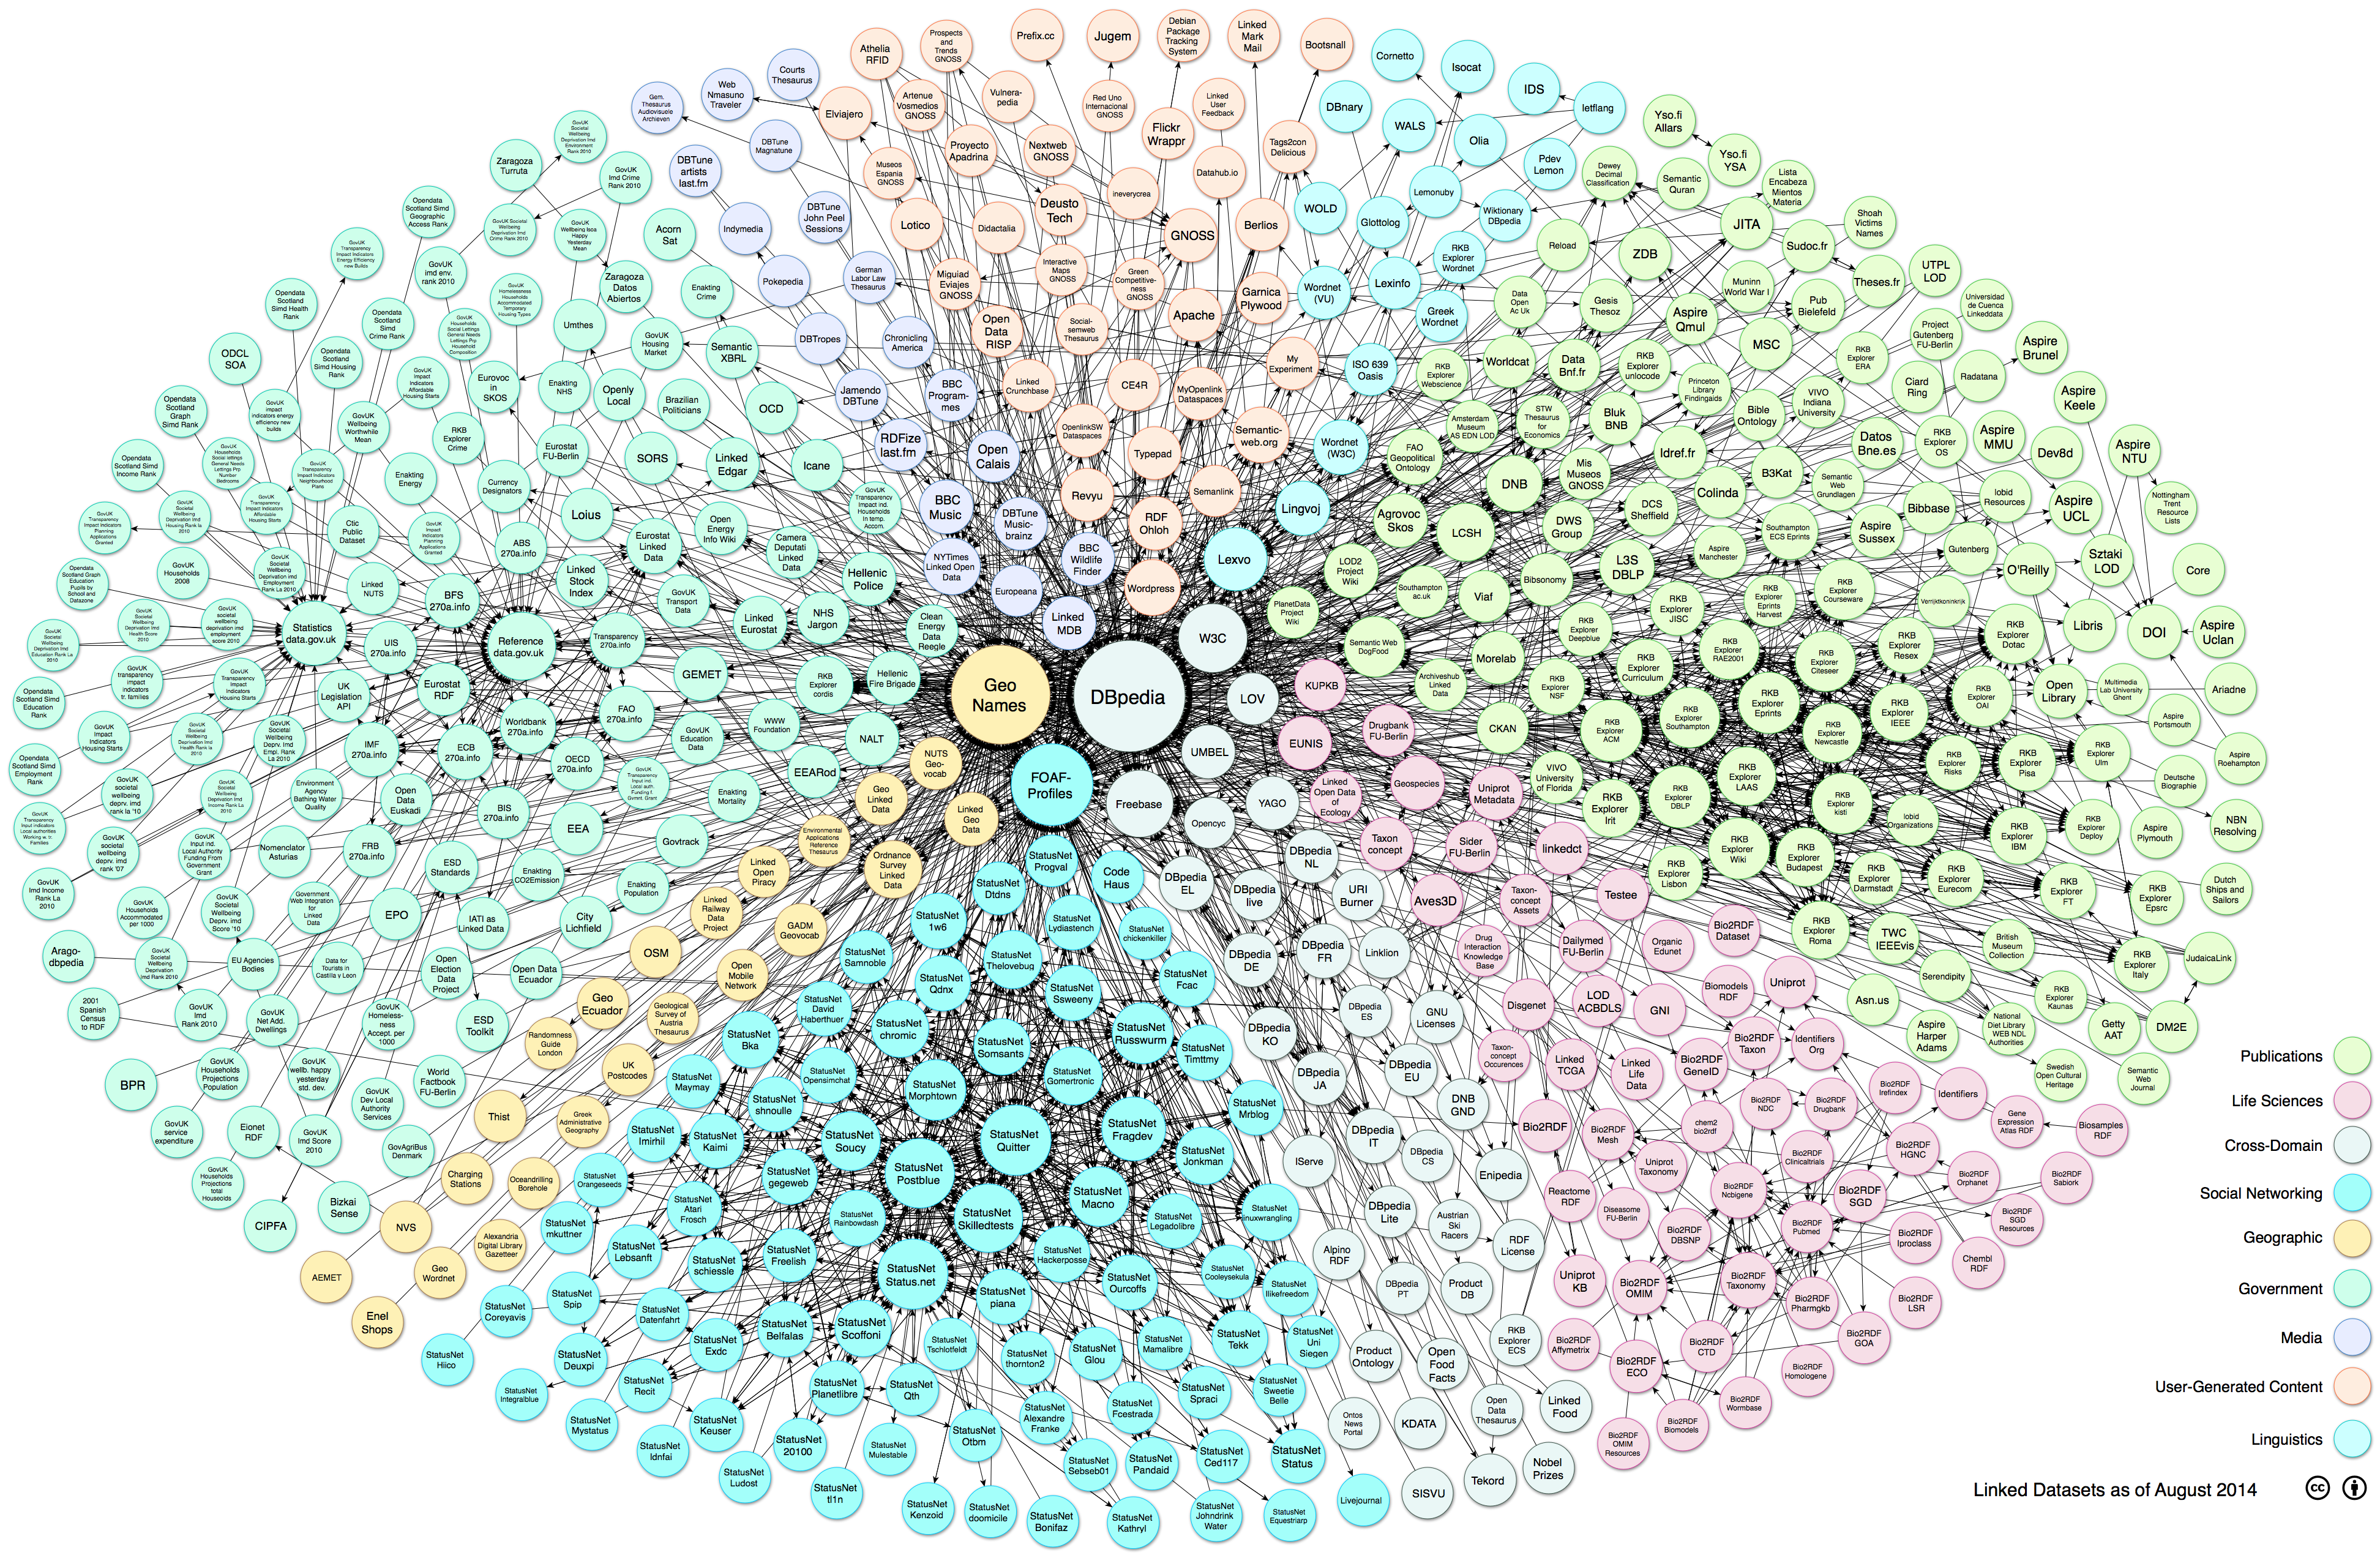
\includegraphics[width=\textwidth]{figures/open_linked_data_could.png}
  \caption{Conexiones entre las bases de datos abiertas hasta agosto del 2014.}
  \vspace{-.2cm}
  \caption*{En morado las bases de datos biológicas, gran parte de ellas son
  parte del proyecto Bio2RDF.}
  \vspace{-.2cm}
  \caption*{Creado por Linked Open Data Cloud project\cite{lod:cloud}.}
  \label{fig:cloud}
\end{figure}
~\vspace{-1cm}
\section{Identificación del problema}

El proyecto Bio2RDF (en su versión 3) incorpora la información de 35 bases de
datos RDF con información biológica, cerca de 11.000 millones de triples que
conforman la red de data enlazada más grande de esta ciencia.

Debido al volumen de datos que se manejan en este proyecto se hace interesante
determinar cual es la información más consultada por parte de los usuarios y 
así verificar que ésta tenga el soporte adecuado en el modelo. 
Para ello es indispensable contar con métricas que analicen el uso de los datos
consultados y la relación entre los mismos.

Si bien en trabajos anteriores como en Hu \emph{et al.}\cite{hu2015link} se han
determinado parámetros como el grado de distribución, la simetría y la
transitividad de los enlaces entre las diferentes bases de datos, no existe un
estudio que determine cual es el subconjunto de datos que realmente son
consultados por los usuarios y la relación entre estos y por ello no es posible
verificar cuales son las entidades más importantes dentro del proyecto Bio2RDF.

Se ha determinado (\hspace{1sp}\cite{hu2015link}) que los enlaces entre
las bases de datos de Bio2RDF presentan el fenómeno de ``mundo pequeño'' lo cual
indica que, a pesar del gran número de nodos que existen en esta red de datos,
generalmente es posible encontrar un camino relativamente corto entre ellos.
Este fenómeno se presenta generalmente en las redes sociales donde se
teoriza que dos individuos cualquiera están relacionados entre si por un número
pequeño de pasos, como describe la hipótesis de los seis grados de separación o
muestra el estudio ``Anatomy of Facebook''\cite{ugander2011anatomy}.

Debido a estas características consideramos atractivo generar un cálculo de
centralidad para los datos consultados por los usuarios al proyecto Bio2RDF,
específicamente a la base de datos que presenta mayor cantidad de consultas en
él: DrugBank, y de esta manera identificar cuales son las instancias más
importantes dentro de esta base de datos.

\section{Objetivos}

El objetivo de este trabajo es generar estadísticas de centralidad sobre el
subconjunto de datos consultados por los usuarios al proyecto Bio2RDF,
particularmente a la base de datos con más consultas en él: DrugBank y comparar
estos resultados con el modelo del proyecto en sí.

\subsection{Objetivos específicos}
Para el logro del objetivo general se plantean los siguientes objetivos
específicos:
\begin{enumerate}
  \item
    Generar un subgrafo del proyecto Bio2RDF a través del análisis de las
    consultas SPARQL hechas al servidor por parte de los usuarios en un periodo
    de tiempo determinado.
  \item
    Analizar el grafo generado por medio de métricas de centralidad para grafos.
  \item
    Comparar los resultados del estudio con el proyecto Bio2RDF.
\end{enumerate}

%!TEX root = main.tex

\chapter{Estado del arte}
El proyecto Bio2RDF utiliza las tecnologías de la Web Semántica para su
implementación y funcionamiento. Así, el análisis que se hará en esta memoria
toma estos conocimientos como base y generará a través de ellos estadísticas de
centralidad con las cuales se determinará cuales son los datos más importantes
de dicha base de datos.

Para poder analizar el problema correctamente es necesario el conocimiento de
las tecnologías que se enuncian en este capítulo. En la sección \ref{ea:ws} se
describe qué es la Web Semántica y las tecnologías que la componen.
En la sección \ref{ea:bio} se hace una revisión al proyecto Bio2RDF y a las
bases de datos que forman parte de él, en especial a la utilizada en este
documento: DrugBank; y en la sección \ref{ea:cent} se repasan conceptos básicos
de teoría de grafos y se introduce el concepto de centralidad junto a sus
métricas y algoritmos.

\section{Web Semántica}\label{ea:ws}
La Web Semántica es un conjunto de actividades propuestas por la \emph{World
Wide Web Consortium} (desde ahora W3C) con el objetivo de generar tecnologías
para la publicación de datos en la web de tal manera que sean procesables por
las maquinas. 
Se basa en la idea de añadir metadatos semánticos y ontológicos que describan el
contenido y la relación entre los datos publicados.
De esta manera se logra mejorar la interoperatividad de internet pues los
programas podrán acceder a la información en un lenguaje que comparte el mismo 
vocabulario y modelo de datos, para así procesar su contenido, razonar en base a
éste y combinarlo para resolver problemas cotidianos automáticamente.

Es posible rastrear los orígenes de esta idea hasta una propuesta temprana de la
\emph{World Wide Web} en 1986~\cite{berners1989proposal} y el subsecuente
trabajo de Berners-Lee \etal\cite{berners1992world} donde se prevé la
necesidad de una evolución desde objetos legible por las personas a información
semántica orientada a las máquinas.

Para lograr los objetivos de la Web Semántica se han generado múltiples
metalenguajes y estándares de representación como son XML, XML Schema, RDF,
RDF Schema, OWL y SPARQL. Estas tecnologías se utilizan actualmente para generar
datos enlazados (\emph{Linked Data}), que buscan enlazar información arbitraria
en la web generando así una ``\emph{red de las cosas del mundo, descrita por los
datos en la Web}''\cite{berners2011linked}.

\begin{figure}[htpb]
  \centering
  \includegraphics[width=.58\textwidth]{figures/Semantic_web_stack.png}
  \caption{Pila de tecnologías de la Web Semántica.}
  \vspace{-.25cm}
  \caption*{De \emph{Semantic Web - XML2000} - Tim
            Berners-Lee\cite{img:swstack}.}
  \label{fig:swstack}
\end{figure}

En las siguientes secciones se describirán más detalladamente algunos de los
conceptos presentados en la figura \ref{fig:swstack} comenzando desde la base,
con las tecnologías del hipertexto (URI y XML), para luego pasar a las
tecnologías de la Web Semántica más estandarizadas (RDF, RDFS y OWL) y terminar
con el lenguaje de consulta SPARQL.

\subsection{URI}
Una URI (del las siglas del ingles \emph{Uniform Resource Identifier}) es una
cadena de caracteres utilizada para identificar un recurso inequívocamente.
Si bien en un principio solo acepta un subconjunto caracteres ASCII (el alfabeto
en ingles y los números) y ``código porciento'' (en el cual, por ejemplo '\%26'
es '\&') el estándar fue extendido el 2005 a IRI (\emph{Internationalized
resource identifier}) que puede contener caracteres Unicode/ISO 10646,
incluyendo chino, japones, koreano, entre otros\cite{gangemi2006bourne}.
En este documento no se diferenciará entre URI e IRI.

La sintaxis actual de una URI fue definida por Berners-Lee et al. el
2005 ~\cite{berners2004uniform} como sigue:\\
\texttt{
  scheme:{[//{[user:passwd@]}host{[:port]}]}{[/]}path{[?query]}{[\#frag]}
}\\
donde:
\begin{itemize}
  \item
    El \bf{esquema} (\emph{scheme}) que consiste en una secuencia de caracteres
    sensibles a las mayúsculas que comienza con una letra y es seguido por
    cualquier combinación de letras, puntos (\tt{.}), guiones (\tt{-}) y signos
    más (\tt{+}), terminando con dos puntos (\tt{:}). 
    Ejemplos populares son \tt{http:}, \tt{ftp:} y \tt{mailto:}.
  \item
    Las dos barras (\tt{//}) son requeridos para algunos esquemas. Cuando la
    componente de autoridad no está presente la ruta no puede comenzar con dos
    barras.
  \item
    La \bf{autoridad} se divide como sigue:
    \begin{itemize}
      \item
        Una \bf{autentificación} opcional compuesta por el usuario
        (\emph{user}), dos puntos y una contraseña (\emph{password}) terminando
        en un arroba (\tt{@}).
      \item
        Un anfitrión (\emph{host}) que puede ser un nombre registrado un una
        dirección IP.
      \item
        Un número de \bf{puerto} opcional (\emph{port}) separado del anfitrión
        por dos puntos.
    \end{itemize}
  \item
    Una \bf{ruta} (\emph{path}) que es una secuencia de segmentos separados
    por una barra (\tt{/}) que comienza con una de las mismas. Generalmente
    representa la localización de un archivo en un sistema de archivos
    jerárquico pero no es necesario.
  \item
    Una \bf{consulta} opcional (\emph{query}) que comienza con un signo de
    interrogación (\tt{?}) y, a pesar de no tener un sintaxis claramente
    definida, usualmente presenta pares atributo-valor.
  \item
    Un \bf{fragmento} opcional (\emph{fragment}) que comienza con un numeral
    (\tt{\#}) seguido por un identificador secundario al recurso principal.
\end{itemize}

\begin{figure}[htpb]
  $$
    \underbrace{\text{http}}_{\text{esquema}}\text{://}
    \overbrace{
      \overbrace{
        \underbrace{\text{user:password}}_{\text{autentificación}}\text{@}
        \underbrace{\text{example.com}}_{\text{anfitrión}}\text{:}
        \underbrace{\text{80}}_{\text{puerto}}
      }^{\text{autoridad}}
      \overbrace{\text{/path/data}}^{\text{ruta}}
    }^{\text{parte jerárquica}}\text{?}
    \underbrace{\text{key=value}}_{\text{consulta}}\text{\#}
    \underbrace{\text{section1}}_{\text{fragmento}}
  $$
  \caption{Ejemplo de una URI.}
  \label{fig:uriex}
\end{figure}

Un ejemplo de lo anterior sería la figura \ref{fig:uriex} donde podemos notar
que una URL (\emph{Uniform Resource Locator}) es una URI, pero no debemos
confundir los términos pues una URL además de identificar un recurso web permite
obtener una representación del mismo generalmente en formato HTML vía HTTP. Es
decir, una URL es una URI que apunta a un recurso físico en la web, mientras que
una URI no necesariamente debe apuntar a una localización que exista realmente.

\subsection{XML}
XML es el acrónimo del ingles \emph{Extensible Markup Language}. Es un
lenguaje de marcado desarrollado por el W3C para almacenar datos de manera
legible tanto por personas como por máquinas. 
El diseño de XML busca la simplicidad, generalidad y usabilidad a través de
internet\cite{paoli2004extensible}. 

Un documento XML puede comenzar con un identificador declarando alguna
información sobre el documento en sí. Luego el cuerpo del fichero debe contener
solo un elemento raíz y dentro de éste se pueden escribir múltiples elementos y
atributos.

\begin{figure}[htpb]
  \centering
  \begin{tabular}{c}
    \lstinputlisting[
      basicstyle=\ttfamily\scriptsize,
      language=xml]{code/example-xml.xml}
  \end{tabular}
  \caption{Ejemplo de XML.}
  \vspace{-.25cm}
  \label{fig:xmlex}
\end{figure}

En la figura~\ref{fig:xmlex} vemos la libertad que nos da XML a la hora de
representar cualquier tipo de información, pero esta libertad hace que
interpretar la validez de un documento sea complicado, pues la información
contenida en este puede ser sensible a la aplicación y el lenguaje definido con
esta tecnología. En respuesta a esta problemática el W3C desarrolló \emph{XML
Schema} que cobra vital importancia para la Web Semántica.

\subsection{XSD}
XSD (del ingles \emph{XML Schema Definition}) es una recomendación del W3C que
especifica formalmente la estructura y restricciones de los contenidos de un
fichero XML de manera precisa más allá de las normas sintácticas del propio
lenguaje XML.

A diferencia de otros lenguajes de esquemas para XML, XSD especifica también
tipos de datos y sus restricciones, logrando un estándar a la hora de
representar datos~\cite{biron2004xml}. 
Presenta 19 tipos de datos básicos: \tt{anyURI},
\tt{base64Binary}, \tt{boolean}, \tt{date}, \tt{dateTime}, \tt{decimal},
\tt{double}, \tt{duration}, \tt{float}, \tt{hexBinary}, \tt{gDay}, \tt{gMonth},
\tt{gMonthDay}, \tt{gYear}, \tt{gYearMonth}, \tt{NOTATION}, \tt{QName},
\tt{string} y \tt{time}. Además permite la creación de nuevos tipos de datos por
medio de tres mecanismos:
\begin{itemize}
  \item \bf{Restricción:} Reduce los valores que puede tomar un dato.
  \item \bf{Lista:} Permite una secuencia de valores.
  \item \bf{Unión:} Permite la elección de valores de diferentes tipos.
\end{itemize}

Gracias a estos factores un fichero XML Schema puede representar un modelo de
datos completo y robusto, con relaciones entre las entidades y asignaciones de 
tipos de datos básicos. La figura~\ref{fig:xsdex} muestra un ejemplo del uso de
XML en conjunto con XSD.

Esta característica es fundamental para la Web Semántica pues todos los tipos de
datos de XSD son compatibles con RDF.

\begin{figure}[htpb]
  \centering
  \begin{tabular}{c}
    \lstinputlisting[
      basicstyle=\ttfamily\scriptsize,
      language=xml]{code/example-xmls.xml}
  \end{tabular}
  \caption{Ejemplo de XMLS.}
  \vspace{-.25cm}
  \caption*{Definiendo una película con XSD.}
  \label{fig:xsdex}
\end{figure}

\subsection{RDF}\label{sw:rdf}
RDF (del inglés \emph{Resource Description Framework}) es una familia de
especificaciones del W3C diseñada como un modelo de datos para metadatos.
Fue adoptado como una recomendación del W3C en 1999, mientras que la
especificación 1.0 fue publicada el 2004 y la 1.1 el
2014\cite{bikakis2013semantic}.

El modelo de datos RDF se basa en la idea de hacer declaraciones sobre 
recursos web (URIs) en forma de expresiones $\langle sujeto, predicado, objeto
\rangle$ que son llamados triples RDF.
El $sujeto$ indica el recurso mientras que el $predicado$ denota la relación
con el $objeto$.
Digamos $U$ un conjunto de URIs, $B$ un conjunto de recursos anónimos y $L$ un
conjunto de literales XSD, podemos denotar un triple RDF como 
$\langle s,p,o\rangle \in (U\cup B) \times U \times (U\cup B\cup L)$.
Así podemos decir que un triple RDF sigue la clásica notación \tt{entidad} - 
\tt{atributo} - \tt{valor} de los modelos orientados a objetos, permitiendo
además, gracias a su simpleza, modelar todo tipo de conceptos abstractos.

Llamaremos vocabulario a la definición de conceptos y relaciones (términos)
utilizados para describir y representar un área de conocimiento.
Otro concepto a tener en cuenta son las ontologías, aunque no existe una clara 
división entre éstas y los vocabularios, generalmente se les considera más
complejas y formales.
En la Web Semántica una colección de triples RDF puede denotar un vocabulario o
ontología.

El vocabulario incluido en la especificación RDF es muy básico y por ello fue
extendido a \emph{RDF Schema}, por lo que la gran mayoría de las bases de datos
RDF actuales contienen ambos vocabularios.

Un conjunto de triples RDF será representado naturalmente por un grafo dirigido.
Esta característica faculta la tecnología para ser parte fundamental de la web 
semántica pues permite relacionar información de diferentes fuentes sin mayor
problema y representarla en un esquema fácilmente identificable.

RDF es un modelo abstracto con varios formatos de serialización, por lo que la
codificación de un triple varía dependiendo el tipo de archivo en el que se
guarde. En esta memoria se trabajará con triples codificados en RDF/XML,
Turtle\cite{beckett2014turtle} y N-Triples\cite{beckett2014nt}.

RDF/XML fue la primera codificación estándar para serializar RDF (en un archivo
XML) y si bien es potente, es difícil de leer por las personas. En base a esto
utilizaremos Turtle y N-Triples pues su simpleza los hace ideales para el
entendimiento y procesamiento de los triples.

Algunas de las reglas para escribir un archivo Turtle (\tt{.ttl}) son las
siguientes:
\begin{itemize}
  \item Toda sentencia termina con un punto (\tt{.}).
  \item La sucesión de tres URIs es un triple.
  \item 
    Si una linea termina en punto y coma (\tt{;}) la siguiente linea mantiene el
    $sujeto$ y solo es necesario escribir las URIs del $predicado$ y el
    $objeto$.
  \item 
    Se pueden definir prefijos con \tt{@prefix rdf: <some\_URI> .}. Esta
    característica es particularmente útil para agregar vocabularios ya
    definidos.
\end{itemize}

N-Triples es una subsección del lenguaje Turtle y su característica principal es
la facilidad que presenta a la hora de analizar su sintaxis. En un archivo
N-Triples (\tt{.nt}) solo se pueden escribir tres URIs seguidas de un punto para
representar un triple RDF y todo lo que esté después de un numeral (\tt{\#}) se
considera un comentario.

Podemos encontrar una descripción completa de las características y sintaxis de
Turtle en~\cite{beckett2014turtle}, de N-Triples en~\cite{beckett2014nt} y de
RDF/XML en ~\cite{beckett2004rdf}.

En la figura \ref{fig:triples} podemos ver un ejemplo básico de la utilización 
de Turtle para la generación de triples (figura \ref{fig:triples:ttl}), el
mismo ejemplo escrito en XML/RDF (figura \ref{fig:triples:rdf}) y como estos
pueden ser visualizados como un grafo dirigido (\ref{fig:triples:grafo}).
\begin{figure}[htpb]
  \centering
  \begin{subfigure}[b]{\textwidth}
    \centering
    \begin{tabular}{c}
      \lstinputlisting[basicstyle=\ttfamily\scriptsize]{
        code/example-turtle.ttl}
    \end{tabular}
    \caption{Ejemplo en Turtle.}
    \label{fig:triples:ttl}
  \end{subfigure}
  \\[0.5cm]
  \begin{subfigure}[b]{\textwidth}
    \centering
    \begin{tabular}{c}
      \lstinputlisting[basicstyle=\ttfamily\scriptsize]{
        code/example-xml-rdf.rdf}
    \end{tabular}
    \caption{Mismo ejemplo en XML/RDF.}
    \label{fig:triples:rdf}
  \end{subfigure}
  \\[0.5cm]
  \begin{subfigure}[]{\textwidth}
    \centering
    \begin{tikzpicture}
  \begin{scope}[every node/.style={ellipse,thick,draw,font=\small}]
    \node (A) at (0,0)    {ex:utfsm};
    \node (B) at (6,1.5)  {ex:universidad};
    \node (C) at (6,0)    {ex:federico};
    \node (D) at (6,-1.5) {http://www.usm.cl};
    \node (E) at (12.5,0) {Federico Santa Maria};
  \end{scope}
  \begin{scope}[>={Stealth[black]},
                every node/.style={font=\footnotesize},
                every edge/.style={draw=black,very thick}]
    \path[->] (A) edge [sloped, above]   node {rdf:type}      (B);
    \path[->] (A) edge [above]           node {ex:fundador}   (C);
    \path[->] (A) edge [sloped, below]   node {ex:pagina}     (D);
    \path[->] (C) edge [above, pos=0.45] node {ex:nombre}     (E);
  \end{scope}
\end{tikzpicture}

\begin{tikzpicture}
  \begin{scope}[every node/.style={ellipse,thick,draw,font=\small}]
    \node (A) at (0,0)  {ex:fundador};
    \node (B) at (0,-1.5) {ex:nombre};
    \node (C) at (5,-0.75) {rdf:Property};
  \end{scope}
  \begin{scope}[>={Stealth[black]},
                every node/.style={font=\footnotesize},
                every edge/.style={draw=black,very thick}]
    \path[->] (A) edge [sloped, above]   node {rdf:type}      (C);
    \path[->] (B) edge [sloped, above]   node {rdf:type}      (C);
  \end{scope}
\end{tikzpicture}

    \caption{Grafo generado.}
    \label{fig:triples:grafo}
  \end{subfigure}
  \caption{Ejemplo de triples RDF.}\label{fig:triples}
\end{figure}

\subsection{RDFS}
RDFS (de las siglas del ingles \emph{Resource Description Framework Schema},
también llamado RDF Schema) es un vocabulario que extiende RDF proveyendo un
set de clases y propiedades que mejoran la creación de modelos como son:
\tt{Class} para declarar clases, \tt{subClassOf} para denotar herencia,
\tt{range} y \tt{domain} para el rango y dominio de cierta propiedad
(\tt{rdf:Property}), entre otras.

RDF fue presentado en 1998 e introducido finalmente como recomendación del W3C
el 2004\cite{bikakis2013semantic}.

RDFS provee el vocabulario necesario para la construcción de cualquier ontología
más avanzada y por ello es la base de otros vocabularios del como OWL y SKOS.

La especificación completa del vocabulario puede encontrarse en ~\cite{brickley2014rdfs}.
%en https://en.wikipedia.org/wiki/RDF_Schema#RDFS_entailment hay un ejemplo.

\subsection{OWL}
OWL (del ingles \emph{Web Ontology Language}) es una familia de lenguajes para
la creación de ontologías complejas.
Agrega lógica computacional para que las relaciones
hechas con este lenguaje puedan ser procesadas con el fin de verificar la
consistencia de la información o generar información implicita.

La versión actual de OWL se conoce como ``OWL 2'' y fue publicada el 2009 como 
una revisión y extensión de la versión inicial publicada el
2004\cite{bikakis2013semantic}. Generalmente cuando se hablar de ``OWL'' nos
referimos a la versión del 2004.

Actualmente OWL tiene tres variantes (sublenguajes) enumerados del más simple al
más complejo como sigue\cite{mcguiness2004owl}:
\begin{enumerate}
  \item \bf{OWL Lite}:
    Se ideó pensando en dar soporte a restricciones simples y jerarquía básica,
    por ejemplo la cardinalidad de los números. 
    Se esperaba que fuera más facil generar y mantener herramientas para OWL
    Lite que para sus variantes más avanzadas, pero debido a que casi todas las
    características de OWL DL pueden ser implementadas como una combinación de
    las de OWL Lite, los desarrolladores han probado que no es 
    así\cite{grau2008owl}. Actualmente OWL Lite no es ampliamente utilizado.
  \item \bf{OWL DL}:
    Fue diseñado para proveer la máxima expresividad posible sin perder la
    decidibilidad y completitud computacional. Posee el vocabulario completo de
    OWL pero solo puede ser utilizado cumpliendo ciertas restricciones.
  \item \bf{OWL Full}:
    Fue diseñado para mantener la compatibilidad con RDFS, permite todo el
    vocabulario sin restricciones pero es indecidible por lo que un programa de
    razonamiento no puede asegurar la completitud de los resultados.
\end{enumerate}
Así, toda ontología o conclusión valida en OWL Lite tambien lo será en OWL DL y
estás a su vez lo serán en OWL Full.

OWL 2 tiene tres perfiles dependiendo de la función que cumple.
\begin{enumerate}
  \item \bf{OWL 2 EL}: 
    Es el fragmento del lenguaje decidible en tiempo polinomial, diseñado para
    trabajar con grandes volúmenes de propiedades y clases.
  \item \bf{OWL 2 QL}:
    Fue diseñado para facilitar el acceso a \emph{datasets} con un gran número
    de instancias donde las consultas son más importantes que el razonamiento.
  \item \bf{OWL 2 RL}:
    Está optimizado para el análisis de reglas lógicas, en aplicaciones que
    requieren un razonamiento escalable sin perder la expresividad del lenguaje.
\end{enumerate}
Se pueden ver las características completas de los perfiles de OWL 2 en
~\cite{motik2009owlprofiles}.

\subsection{SPARQL}
SPARQL (del ingles \emph{SPARQL Protocol and RDF Query Language}) es un lenguaje
estandarizado para consultar grafos RDF, se constituyó como una recomendación
oficial por la W3C en el 2008\cite{bikakis2013semantic}. La versión actual de
SPARQL es la 1.1\cite{world2013sparql}.

SPARQL provee un set completo de operaciones analíticas para sus consultas
definidas directamente en la especificación. Particularmente provee 4 formas de
consultas:
\begin{itemize}
  \item \bf{\tt{SELECT}}:
    Retorna valores en forma de tabla.
  \item \bf{\tt{CONSTRUCT}}:
    Retorna valores en forma de triples RDF.
  \item \bf{\tt{ASK}}:
    Retorna un resultado binario a la consulta (\tt{True/False}).
  \item \bf{\tt{DESCRIBE}}:
    Retorna un grafo RDF con contenido que el administrador del \emph{endpoint}
    SPARQL considere información útil.
\end{itemize}
A excepción de \tt{DESCRIBE}, las demás consultas necesitan un bloque \tt{WHERE}
con sintaxis similar a Turtle en el cual se determinan las restricciones de la
búsqueda en forma de triples RDF con variables y URIs.

Además de las consultas, SPARQL provee múltiples funciones como son 
las condicionales (\tt{if}, \tt{exists}, etc), de conversión (\tt{str},
\tt{lang}, etc), de comprobación (\tt{isNumber}, \tt{isBlank}, etc) y
modificadores de respuesta como \tt{ORDER BY}, \tt{DINSTINCT}, \tt{REDUCED},
\tt{LIMIT} y \tt{OFFSET}. Una descripción completa del lenguaje puede
encontrarse en~\cite{prud2008sparql} y en~\cite{world2013sparql}, mientras que 
en~\cite{perez2006semantics} se estudia la lógica de conjuntos y complejidad del
mismo.

\begin{figure}[htpb]
  \centering
  \begin{subfigure}[b]{\textwidth}
    \centering
    \begin{tabular}{c}
      \lstinputlisting[basicstyle=\ttfamily\scriptsize]{
        code/example-select.sparql}
    \end{tabular}
    \caption{Ejemplo de consulta tipo \tt{SELECT}.}
    \label{fig:sparql:select}
  \end{subfigure}
  \\[0.5cm]
  \begin{subfigure}[b]{\textwidth}
    \centering
    \begin{tabular}{c}
      \lstinputlisting[basicstyle=\ttfamily\scriptsize]{
        code/example-construct.sparql}
    \end{tabular}
    \caption{Ejemplo de consulta tipo \tt{CONSTRUCT}.}
    \label{fig:sparql:construct}
  \end{subfigure}
  \caption{Ejemplo de consultas SPARQL.}\label{fig:sparql}
\end{figure}

En la figura~\ref{fig:sparql:select} se ve un ejemplo de una consulta SPARQL al
\emph{endpoint} de DBpedia\footnote{\url{http://dbpedia.org/sparql}}, en ella se
preguntan todas las películas, actores y directores en los cuales se cumpla que
el director también es productor y el actor es su hijo. La consulta retornará a
lo más 100 resultados y estos serán representados en una tabla con tres
columnas: ``pelicula'' ``actor'' y ``director''.

Por otro lado en la figura~\ref{fig:sparql:construct} se hace la misma consulta,
pero los resultados serán triples RDF con las relaciones especificadas, entre
las cuales solo se guarda la fuente de la información como la cadena de
caracteres ``dbpedia'' y al actor y director como participantes de la película.

Podemos notar como la consulta \tt{CONSTRUCT} posee la capacidad de generar
nueva información con base a los resultados de una búsqueda y no se limita
solamente a las relaciones ya existentes, gracias a ello se pueden formar
triples RDF relativamente simples de consultas mucho más complejas. Por otro
lado, si solo se busca retornar la información en formato RDF no es necesario
que la clausula tenga argumentos (\tt{CONSTRUCT WHERE \{...\}} ), aunque este
método no funcionará con consultas más complejas como aquellas con triples
opcionales.

\newpage %FIXME
\section{Proyecto Bio2RDF}\label{ea:bio}
Bio2RDF\hspace{0.5mm}\footnote{\url{http://bio2rdf.org/}}
\cite{belleau2008bio2rdf,callahan2013bio2rdf} es un proyecto de código
abierto que utiliza las tecnologías de la Web Semántica para construir la
red más grande de datos enlazados de las ciencias biológicas.
El proyecto reúne 35 bases de datos en una ontología común generando enlaces
entre ellos.

La tabla~\ref{tab:bio2RDFdataset} muestra el número de entidades y sus
relaciones para cada integrante del proyecto, mientras que la
figura~\ref{fig:bio2rdfgraph} muestra una representación de cada
base de datos como un nodo del grafo y sus respectivos arcos están determinados
por la cantidad de enlaces entre sus entidades.
Ambos esquemas son de la \emph{release} 3, la cual data de julio del 2014 y es
la versión que se mantiene en linea.
Versiones más recientes pueden ser descargadas directamente de la pagina web.

\begin{table}[htpb]
\centering
\begin{tabular}{|c|l|r|r|}
  \hline
  \bf{\#} & \bf{Dataset} & \bf{Triples} & \bf{Entities} \\\hline
  01 & affymetrix     &   86942 &   6680\\\hline
  02 & biomodels      &    2380 &    188\\\hline
  03 & bioportal      &   19920 &   2200\\\hline
  04 & chembl         &  409942 &  50061\\\hline
  05 & clinicaltrials &   98836 &   7337\\\hline
  06 & ctd            &  326721 &  19769\\\hline
  07 & dbsnp          &  8801,4 &  530,5\\\hline
  08 & \bf{drugbank}  &  3672,5 &  316,9\\\hline
  09 & genage         &      73 &    6,9\\\hline
  10 & gendr          &    11,6 &    1,1\\\hline
  11 & goa            &   97520 &   5950\\\hline
  12 & hgnc           &    3628 &  372,1\\\hline
  13 & homologene     &    7190 &  869,9\\\hline
  14 & interpro       &    2323 &  176,5\\\hline
  15 & iproclass      & 3306107 & 364255\\\hline
  16 & irefindex      &   48782 &   3111\\\hline
  17 & kegg           &   50197 &   6533\\\hline
  18 & linkedspl      &  2174,5 &   59,7\\\hline
\end{tabular}
\hspace{1mm}
\begin{tabular}{|c|l|r|r|}
  \hline
  \bf{\#} & \bf{Dataset} & \bf{Triples} & \bf{Entities} \\\hline
  19 & lsr         &     55,9 &       5\\\hline
  20 & mesh        &   7323,8 &   305,4\\\hline
  21 & mgi         &   8206,8 &   924,2\\\hline
  22 & ncbigene    &  2010284 &  189594\\\hline
  23 & ndc         &   6199,4 &   488,1\\\hline
  24 & omim        &   8750,7 &    1013\\\hline
  25 & orphanet    &    377,9 &    28,8\\\hline
  26 & pathwaycom  &   5700,7 &    1024\\\hline
  27 & pharmgkb    &   278049 &   25325\\\hline
  28 & pubmed      &  5005343 &  412594\\\hline
  29 & reactome    &  12487,4 &    2461\\\hline
  30 & sabiork     &   2716,4 &   448,2\\\hline
  31 & sgd         &  12494,9 &   957,5\\\hline
  32 & sider       &  17627,8 &    1222\\\hline
  33 & taxonomy    &  21310,3 &    1147\\\hline
  34 & wikipathway &    514,4 &    71,8\\\hline
  35 & wormbase    &    22682 &    1840\\\hline
  -- & \bf{total}  & 11895349 & 1107871\\\hline
\end{tabular}
\caption{Datasets del proyecto Bio2RDF y triples y entidades (en miles).}
\vspace{-.2cm}
\caption*{
  Extraído de la página web del proyecto.
}
\label{tab:bio2RDFdataset}
\end{table}


\begin{figure}[htpb]
  \centering
  \includegraphics[page=1,viewport=138 412 480 630,clip]{figures/bio2rdf_graph.pdf}
  \caption{Grafo de las bases de datos del proyecto Bio2RDF.}
  \vspace{-.3cm}
  \caption*{Extraído de \cite{hu2015link}.}
  \label{fig:bio2rdfgraph}
\end{figure}

La base de datos sobre la cual se trabaja en este documento es
Drugbank\cite{wishart2006drugbank} debido a la gran cantidad de consultas que
presenta y el tipo de datos que maneja. Según su página
web\footnote{\url{http://www.drugbank.ca/}}, DrugBank es una base de datos única
en la bioinformática que combina detallados datos sobre drogas (químicas,
farmacológicas, farmacéuticas, etc) e información exhaustiva de las mismas
(secuencia, estructura, etc).

En \cite{hu2015link} podemos encontrar estadísticas sobre el modelo de datos
hecho para el proyecto Bio2RDF. Entre las conclusiones relevantes se destaca:
\begin{itemize}
  \item
    Se produce el fenómeno de mundo pequeño, lo que denota una gran
    conectividad. (\emph{small world phenomenom}).
  \item
    La distribución de las relaciones no sigue una ley potencial.
  \item
    La simetría y transitividad no logran traspasar las fronteras de la propia
    base de datos.
\end{itemize}

Información sobre los \emph{endpoint} SPARQL para hacer consultas al proyecto
puede ser encontrada en \cite{callahan2013bio2rdf}.

\section{Centralidad en grafos}\label{ea:cent}
El concepto de centralidad hace referencia a una medida de la importancia
relativa de un nodo en un grafo utilizando su relación con los demás miembros
como base. 
Se puede usar para determinar los caminos más importantes en una ciudad, el
personal clave en una red de trabajo o cualquier fenómeno que pueda ser
representado por nodos y aristas, debido a esto su significado depende del
dominio que estemos representando.

Los orígenes del concepto pueden ser rastreados al trabajo de Bavelas a finales
de los años 1940\cite{bavelas1948mathematical}.
Es uno de los conceptos más relevantes y estudiados para el análisis de redes y
desde finales de los años 70, gracias al trabajo de Freeman 
\etal\cite{freeman1979centrality,freeman1991centrality}, 
cobra nueva importancia en el estudio de las redes sociales.

Desde su definición no existe una noción única para determinar que es realmente 
la centralidad y la forma correcta de medirla\cite{freeman1979centrality},
debido a esto han florecido diferentes técnicas y métodos para ello.

Para entender a cabalidad el concepto las diferentes formas de medirlo es
importante recordar algunas definiciones básicas de teoría de grafos.

\subsection{Grafos}
Un grafo es una abstracción para la representación de datos y sus relaciones en
el cual existen dos elementos fundamentales: los nodos (o vértices), que
representan individuos u objetos, y los arcos (o aristas), que representan las
relaciones entre ellos.
Así, podemos representar una gran variedad de información en este esquema, por
ejemplo, podemos crear un grafo donde cada nodo sea una ciudad y cada arco
sea el camino que existe entre ellas. También podemos representar una red
social donde cada persona sea un nodo y sus relaciones con los demás individuos
estén inscritas en los arcos.

Digamos $G=(V, E)$ un grafo, con $V$ como el conjunto no vacío de nodos y $E$ el
conjunto de arcos.
Denotaremos un nodo $i$ de dicho grafo como  $V_i \in V$ y un arco entre los
nodos $V_i$ y $V_j$ como la tupla $(V_i, V_j) \in E$.

Generalmente los arcos representan relaciones simétricas y por ello son pares no
ordenados, es decir: $(V_i, V_j) = (V_j, V_i)$, pero este esquema no siempre es
adecuado. Un grado dirigido (o digrafo) en aquel en el cual los arcos son pares
ordenados, es decir $(V_i, V_j) = (V_k, V_l)$ si y sólo si $i=k \land j=l$ y por
lo tanto son adecuados para describir relaciones no simétricas. En un digrafo se
dice que el arco $(V_i, V_j)$ va desde $V_i$ hasta $V_j$ o $V_i$ es el nodo
inicial y $V_j$ el nodo final.

Para un grafo cualquiera se definen los siguientes conceptos (entre otros):
\begin{itemize}
  \item \bf{Orden:}
    Se llama orden del grafo G al número de nodos que lo conforman, generalmente
    se designa como $|V|$.
  \item \bf{Adyacencia:}
    Se dice que el nodo $V_i$ es adyacente al $V_j$ si existe el arco 
    $(V_i, V_j) \in E$. Al conjunto de nodos adyacentes a cierto nodo $V_i$ se
    le llama \bf{vecinos} de $V_i$.
  \item \bf{Grado:}
    El grado de cierto nodo es el número de aristas incidentes a él. Para un
    digrafo podemos distinguir el grado saliente (número de arcos salientes de
    él) y el grado entrante (número de arcos entrantes a él).
  \item \bf{Camino:}
    Se dice que existe un camino entre el nodo $V_i$ y el nodo $V_j$ si existe
    una sucesión de arcos de tal manera que comenzando desde el nodo $V_i$ y
    revisando entre sus vecinos y los vecinos de ellos sucesivamente se logre
    llegar al nodo $V_j$.
  \item \bf{Distancia:}
    Es la cantidad de arcos que conforman un camino.
  \item \bf{Camino más corto:}
    El camino más corto entre $V_i$ y $V_j$ será el camino entre $V_i$ y $V_j$
    con menor distancia.
\end{itemize}

\begin{figure}[htpb]
  \centering
  \begin{tikzpicture}
  \begin{scope}[every node/.style={circle,thick,draw}]
    \node (A) at (0,0)    {A};
    \node (B) at (2,1.5)  {B};
    \node (C) at (2,0)    {C};
    \node (D) at (2,-1.5) {D};
    \node (E) at (4,0)    {E};
    \node (F) at (6,0)    {F};
  \end{scope}
  \begin{scope}[>={Stealth[black]},every edge/.style={draw=black,very thick}]
    \path[->] (A) edge (B);
    \path[->] (A) edge (C);
    \path[->] (B) edge (C);
    \path[->] (C) edge (D);
    \path[->] (C) edge (E);
    \path[->] (D) edge (E);
    \path[->] (F) edge (E);
  \end{scope}
\end{tikzpicture}

  \caption{Ejemplo de digrafo.}
  \label{fig:exgraph}
\end{figure}

Del ejemplo mostrado en la figura~\ref{fig:exgraph} podemos notar lo siguiente:
\begin{itemize}
  \item
    Podemos denotar el grafo como $G = (V,E)$ con los conjuntos 
    $V = \{A,B,C,D,E,F\}$ y 
    $E = \{(A,B),(A,C),(B,C),(C,D),(C,E),(D,E),(F,E)\}$.
  \item 
    El orden de $G$ será $|V| = 6$.
  \item
    El nodo $A$ es adyacente con los nodos $B$ y $C$, es decir: son sus vecinos.
    De forma similar el nodo $E$ no tiene vecinos pues no es nodo inicial de
    ningún arco.
  \item
    El grado saliente del nodo $A$ es $2$, mientras que el entrante es $0$.
    $C$ por su parte tiene grado saliente de $2$ y entrante de $2$.
  \item
    Existen 4 caminos entre $A$ y $E$: $C_1 = \{(A,B),(B,C),(C,D),(D,E)\}$ de
    distancia $4$, $C_2 = \{(A,B),(B,C),(C,E)\}$ de distancia $3$,
    $C_3 = \{(A,C),(C,D),(D,E)\}$ de distancia $3$ y
    $C_4 = \{(A,C),(C,E)\}$ de distancia $2$, claramente éste es el camino más
    corto.
\end{itemize}

\subsection{Tipos de centralidad}
Desde su definición se han propuesto varias medidas de centralidad de un nodo.
Las cuatro que se presentan a continuación son las más ampliamente estudiadas
en el análisis de redes.

Bajo las medidas de centralidad de grado y cercanía se le da mayor importancia a
los nodos y partes del grafo más conectadas con el resto del mismo. Por su parte
la intermediación determina los puntos críticos por donde circula la información
de manera que si se extraen estos nodos se pierde más conectividad en general.
Por último, la centralidad de vector propio determina cuales son los nodos más
importantes para mantener el comportamiento y la forma de una red.

Se pueden distinguir entre medidas absolutas y relativas, las primeras no son
comprables mientras que las segundas están normalizadas, generalmente con base
al nodo más central.

\subsubsection{Centralidad de grado}\label{ea:cent:degree}
La centralidad de grado (en ingles \emph{degree centrality}) es la primera y más
simple medida de centralidad\cite{sun2011survey}.
Se basa en medir el número de arcos existentes para cada nodo, así, se define
como: 
\begin{equation}
  \label{eq:deg}
  C_{DEG}(V_i) = \text{grado}(V_i)
\end{equation}
Si se tiene la matriz de adyacencia ($\mathbb{A}$) la operación se reduce a
calcular el largo de la lista de nodos adyacentes a cada nodo, es decir:
$ C_{DEG}(V_i) = \sum_{j} \mathbb{A}_{i,j}$.

Para digrafos se puede diferenciar entre la centralidad de grado de entrada,
donde se calcula el grado entrante de cada nodo, y la centralidad de grado de
salida, donde se hace lo mismo con el grado saliente. El algoritmo para calcular 
esta centralidad tiene una complejidad computacional de $\Theta (E)$.

\begin{figure}[htpb]
  \begin{equation*}
    \bordermatrix{
       ~  & $A$ & $B$ & $C$ & $D$ & $E$ & $F$ \cr
      $A$ &  0  &  1  &  1  &  0  &  0  &  0  \cr
      $B$ &  0  &  0  &  1  &  0  &  0  &  0  \cr
      $C$ &  0  &  0  &  0  &  1  &  1  &  0  \cr
      $D$ &  0  &  0  &  0  &  0  &  1  &  0  \cr
      $E$ &  0  &  0  &  0  &  0  &  0  &  0  \cr
      $F$ &  0  &  0  &  0  &  0  &  1  &  0  \cr
    }
  \end{equation*}
  \caption{Matriz de adyacencia del grafo de la figura~\ref{fig:exgraph}.}
  \label{fig:adjmatrix}
\end{figure}

A modo de ejemplo la figura~\ref{fig:adjmatrix} presenta la matriz de adyacencia
del grafo de la figura~\ref{fig:exgraph}, ésta facilita el cálculo de
centralidad de grado.

Sumando por filas obtenemos la centralidad de grado saliente, mientras que
sumando por columnas obtenemos la entrante. La tabla~\ref{tab:excgrad} muestra
estos resultados.
\begin{table}[htpb]
  \centering
  \begin{tabular}{|l|c|c|c|c|c|c|}
    \hline
    Centralidad de grado &  A  &  B  &  C  &  D  &  E  &  F  \\\hline
    Entrante             & $0$ & $1$ & $2$ & $1$ & $3$ & $0$ \\\hline
    Saliente             & $2$ & $1$ & $2$ & $1$ & $0$ & $1$ \\\hline
  \end{tabular}
  \caption{Centralidad de grado del grafo de la figura~\ref{fig:exgraph}.}
  \label{tab:excgrad}
\end{table}

Existen varias variantes de esta centralidad, entre ellas se destaca la
centralidad de k~-camino, de Katz, de Bonacich y de Hubbell. Una descripción de
ellas puede ser encontrada en \cite{sun2011survey}.

\subsubsection{Cercanía}
La cercanía (en ingles \emph{closeness centrality}) es una medida de centralidad
introducida por el matemático Beauchamp en 1965\cite{beauchamp1965improved}. Se
basa en calcular la suma o el promedio de las distancias más cortas de todos los
nodos a un nodo en particular. Digamos $d(V_i, V_j)$ como la distancia del
camino más corto entre $V_i$ y $V_j$ ($\infty$ si éste no existe), la cercanía
queda definida como sigue:
\begin{equation}
  \label{eq:far}
  C_{CLO}(V_i) = \sum_{V_j \in V, j\neq i}^{} d(V_j, V_i)
\end{equation}

Si disponemos de la matriz de distancias del grafo ($\mathbb{B}$) la cercanía
se reduce al cálculo de $ C_{CLO}(V_i) = \sum_{j} \mathbb{B}_{ij} $.

Un nodo es más cercano a ser el centro del grafo mientras menor es este valor.
De ello podemos notar que esta definición nos da más bien una noción de
\bf{lejanía}. Este calculo se hace inadecuado para grafos no fuertemente
conexos ya que al tener pocos arcos, la matriz tendrá muchos valores indefinidos
(distancia infinita entre nodos). 

Sabidussi en 1966\cite{sabidussi1966centrality} presenta una definición
de cercanía más conveniente que consiste en calcular el reciproco de la
anterior: 
\begin{equation}
  \label{eq:clo}
  C_{CLO}(V_i) = \sum_{V_j\in V, j\neq i} \frac{1}{d(V_j, V_i)}
\end{equation}

Las figuras~\ref{fig:closs:lej} y \ref{fig:closs:cer} presentan las matrices de
lejanía y cercanía del grafo en~\ref{fig:exgraph}.

\begin{figure}[htpb]
  \centering
  \begin{subfigure}[b]{.4\textwidth}
    \begin{equation*}
      \bordermatrix{
         ~  &   $A$  &   $B$  &   $C$  &   $D$  &   $E$  &   $F$  \cr
        $A$ & -      & 1      & 1      & 2      & 2      & \infty \cr
        $B$ & \infty & -      & 1      & 2      & 2      & \infty \cr
        $C$ & \infty & \infty & -      & 1      & 1      & \infty \cr
        $D$ & \infty & \infty & \infty & -      & 1      & \infty \cr
        $E$ & \infty & \infty & \infty & \infty & -      & \infty \cr
        $F$ & \infty & \infty & \infty & \infty & 1      & -      \cr
      }
    \end{equation*}
    \caption{Matriz de lejanía.}
    \label{fig:closs:lej}
  \end{subfigure}
  \begin{subfigure}[b]{.4\textwidth}
    \begin{equation*}
      \bordermatrix{
       ~  & $A$ & $B$ & $C$ & $D$ & $E$ & $F$ \cr
      $A$ &  -  &  1  &  1  & 0.5 & 0.5 &  0  \cr
      $B$ &  0  &  -  &  1  & 0.5 & 0.5 &  0  \cr
      $C$ &  0  &  0  &  -  &  1  &  1  &  0  \cr
      $D$ &  0  &  0  &  0  &  -  &  1  &  0  \cr
      $E$ &  0  &  0  &  0  &  0  &  -  &  0  \cr
      $F$ &  0  &  0  &  0  &  0  &  1  &  -  \cr
    }
    \end{equation*}
    \caption{Matriz de cercanía.}
    \label{fig:closs:cer}
  \end{subfigure}
  \caption{Matrices de distancia del grafo de la figura~\ref{fig:exgraph}.}
  \label{fig:closs}
\end{figure}


Los resultados de la cercanía según la ecuación~\ref{eq:clo}
quedan plasmados en la tabla~\ref{tab:closeness},
valores mayores indican mayor centralidad. Se muestra demás una normalización
con base al mejor resultado encontrado.
\begin{table}[htpb]
  \centering
  \begin{tabular}{|l|c|c|c|c|c|c|}
    \hline
    Cercanía &  A  &  B  &  C  &  D  &  E  &  F  \\\hline
    Absoluta & $0$ & $1$ & $2$ & $2$ & $4$ & $0$ \\\hline
    Relativa & $0$ & $0.25$ & $0.5$ & $0.5$ & $1$ & $0$ \\\hline
  \end{tabular}
  \caption{Cercanía del grafo de la figura~\ref{fig:exgraph}.}
  \label{tab:closeness}
\end{table}
\vspace{-0.5cm}%FIXME

\subsubsection{Intermediación}\label{ea:cent:bet}
La intermediación (del ingles \emph{betweenness centrality}) cuantifica la
cantidad de veces que cierto nodo es parte del camino más corto entre otros dos
nodos.
La medida fue introducida por Freeman en 1977\cite{freeman1977set} para
cuantificar el control de la comunicación de un humano con otros en una red
social. 

La definición formal de intermediación es la siguiente:
\begin{equation}
  \label{eq:bet}
  C_{BET}(V_v) = \sum_{s\neq v\neq t} \frac{\sigma_{st}(v)}{\sigma_{st}}
\end{equation}
donde $\sigma_{st}$ es el número de caminos más cortos entre $V_s$ y $V_t$ y 
$\sigma_{st}(v)$ es el número de éstos que pasan por el nodo $V_v$.

Para el grafo de~\ref{fig:exgraph} tenemos que la matriz del número de caminos
más cortos (CMC) entre sus nodos será la figura~\ref{fig:nrosp}.

\begin{figure}[htpb]
  \begin{equation*}
    \bordermatrix{
       ~  & $A$ & $B$ & $C$ & $D$ & $E$ & $F$ \cr
      $A$ &  -  &  1  &  1  &  1  &  1  &  0  \cr
      $B$ &  0  &  -  &  1  &  1  &  1  &  0  \cr
      $C$ &  0  &  0  &  -  &  1  &  1  &  0  \cr
      $D$ &  0  &  0  &  0  &  -  &  1  &  0  \cr
      $E$ &  0  &  0  &  0  &  0  &  -  &  0  \cr
      $F$ &  0  &  0  &  0  &  0  &  1  &  -  \cr
    }
  \end{equation*}
  \caption{Número de caminos más cortos del grafo de la figura~\ref{fig:exgraph}.}
  \label{fig:nrosp}
\end{figure}

Además, para el calculo de la intermediación es necesario contar el número de
estos caminos que pasan por cada uno de los nodos.
Este proceso es evidenciado en la figura~\ref{fig:sppn}.

\begin{figure}[htpb]
  \centering
  \begin{subfigure}[b]{.3\textwidth}
    \begin{equation*}
      \bordermatrix{
       ~  & $B$ & $C$ & $D$ & $E$ & $F$ \cr
      $B$ &  -  &  0  &  0  &  0  &  0  \cr
      $C$ &  0  &  -  &  0  &  0  &  0  \cr
      $D$ &  0  &  0  &  -  &  0  &  0  \cr
      $E$ &  0  &  0  &  0  &  -  &  0  \cr
      $F$ &  0  &  0  &  0  &  0  &  -  \cr
    }
    \end{equation*}
    \caption{SP que pasan por A.}
    \label{fig:sppn:a}
  \end{subfigure}
  \hspace{3mm}
  \begin{subfigure}[b]{.3\textwidth}
    \begin{equation*}
      \bordermatrix{
       ~  & $A$ & $C$ & $D$ & $E$ & $F$ \cr
      $A$ &  -  &  0  &  0  &  0  &  0  \cr
      $C$ &  0  &  -  &  0  &  0  &  0  \cr
      $D$ &  0  &  0  &  -  &  0  &  0  \cr
      $E$ &  0  &  0  &  0  &  -  &  0  \cr
      $F$ &  0  &  0  &  0  &  0  &  -  \cr
    }
    \end{equation*}
    \caption{SP que pasan por B.}
    \label{fig:sppn:b}
  \end{subfigure}
  \hspace{3mm}
  \begin{subfigure}[b]{.3\textwidth}
    \begin{equation*}
      \bordermatrix{
       ~  & $A$ & $B$ & $D$ & $E$ & $F$ \cr
      $A$ &  -  &  0  &  1  &  1  &  0  \cr
      $B$ &  0  &  -  &  1  &  1  &  0  \cr
      $D$ &  0  &  0  &  -  &  0  &  0  \cr
      $E$ &  0  &  0  &  0  &  -  &  0  \cr
      $F$ &  0  &  0  &  0  &  0  &  -  \cr
    }
    \end{equation*}
    \caption{SP que pasan por C.}
    \label{fig:sppn:c}
  \end{subfigure}
  \hspace{3mm}
  \begin{subfigure}[b]{.3\textwidth}
    \begin{equation*}
      \bordermatrix{
       ~  & $A$ & $B$ & $C$ & $E$ & $F$ \cr
      $A$ &  -  &  0  &  0  &  0  &  0  \cr
      $B$ &  0  &  -  &  0  &  0  &  0  \cr
      $C$ &  0  &  0  &  -  &  0  &  0  \cr
      $E$ &  0  &  0  &  0  &  -  &  0  \cr
      $F$ &  0  &  0  &  0  &  0  &  -  \cr
    }
    \end{equation*}
    \caption{SP que pasan por D.}
    \label{fig:sppn:d}
  \end{subfigure}
  \hspace{3mm}
  \begin{subfigure}[b]{.3\textwidth}
    \begin{equation*}
      \bordermatrix{
       ~  & $A$ & $B$ & $C$ & $D$ & $F$ \cr
      $A$ &  -  &  0  &  0  &  0  &  0  \cr
      $B$ &  0  &  -  &  0  &  0  &  0  \cr
      $C$ &  0  &  0  &  -  &  0  &  0  \cr
      $D$ &  0  &  0  &  0  &  -  &  0  \cr
      $F$ &  0  &  0  &  0  &  0  &  -  \cr
    }
    \end{equation*}
    \caption{SP que pasan por E.}
    \label{fig:sppn:e}
  \end{subfigure}
  \hspace{3mm}
  \begin{subfigure}[b]{.3\textwidth}
    \begin{equation*}
      \bordermatrix{
       ~  & $A$ & $B$ & $C$ & $D$ & $E$ \cr
      $A$ &  -  &  0  &  0  &  0  &  0  \cr
      $B$ &  0  &  -  &  0  &  0  &  0  \cr
      $C$ &  0  &  0  &  -  &  0  &  0  \cr
      $D$ &  0  &  0  &  0  &  -  &  0  \cr
      $E$ &  0  &  0  &  0  &  0  &  -  \cr
    }
    \end{equation*}
    \caption{SP que pasan por F.}
    \label{fig:sppn:f}
  \end{subfigure}
  \caption{Número de caminos más cortos que pasan por cada nodo del
  grafo~\ref{fig:exgraph}.}
  \label{fig:sppn}
\end{figure}


De la aplicación de la ecuación~\ref{eq:bet} se obtienen los resultados
presentados en la tabla~\ref{tab:exbet}.

\begin{table}[h!]
  \centering
  \begin{tabular}{|l|c|c|c|c|c|c|}
    \hline         &  A  &  B  &  C  &  D  &  E  &  F  \\\hline
    Intermediación & $0$ & $0$ & $4$ & $0$ & $0$ & $0$ \\\hline
  \end{tabular}
  \caption{Intermediación del grafo de la figura~\ref{fig:exgraph}.}
  \label{tab:exbet}
\end{table}

Este proceso, al igual que para el calculo de la cercanía, implica la obtención
de todos los caminos más cortos lo cual conlleva una complejidad computacional
de $\Theta (V^3)$, pero existen algoritmos que aprovechando las características
de los grafos mejoran notablemente este tiempo. Para grafos dispersos podemos
utilizar el algoritmo de Johnson\cite{johnson1977efficient} de complejidad 
$O(V^2\log (V) + VE)$ mientras que para grafos sin pesos en sus arcos se puede
utilizar el algoritmo de Brandes\cite{brandes2001faster} que toma $O(VE)$
tiempo.

Será particularmente útil en este trabajo el algoritmo de Brandes ya que el
grafo con el que se trabajará no tiene pesos en sus arcos. La idea principal es
realizar una búsqueda en anchura para cada nodo e incrementar el número de
caminos más cortos que pasan por todos los nodos visitados. La segunda idea
principal es que $\frac{\sigma_{st}(v)}{\sigma_{st}}$ ($\delta_{st}(v)$) puede
ser obtenido por separado. 
Definamos la \it{dependencia} de un nodo fuente $V_s \in V$ a un nodo $V_v \in
V$ como $\delta_s (v) = \sum_{t\in V}\delta_{st}(v)$ entonces la intermediación
del nodo $V_v$ puede ser expresada como
$C_{BET} (V_v) = \sum_{s\neq v}\delta_s(v)$. Brandes demuestra que los valores
de dependencia satisfacen la siguiente relación recursiva:
\begin{equation}\label{eq:brand}
  \delta_s (v) = \sum_{w:d(s,w) = d(s,v) + 1} \frac{\sigma_{sv}}{\sigma_{sw}}
  (1 + \delta_s(w))
\end{equation}
Así, el calculo de la intermediación para cada nodo se calcula en dos partes,
primero obtenemos la distancia y el camino más corto a todos los demás nodos y
luego, desde el final hacia el principio, se calcula la dependencia según la
ecuación~\ref{eq:brand}.

\subsubsection{Centralidad de vector propio}
La centralidad de vector propio (en ingles \emph{Eigenvector centrality}) fue
introducida en 1972 por Phillip Bonacich\cite{bonacich1972factoring}.
Plantea que los nodos más centrales serán aquellos que están conectados con
muchos nodos que, a su vez, también están bien conectados.
Esta centralidad corresponde al vector propio dominante de la matriz de
adyacencia del grafo analizado. 

Para una matriz de adyacencia $\mathbb{A}$ de cierto grafo $G=(V,E)$ se definen 
los valores ($\lambda$) y vectores ($\vec{v}$) propios como aquellos que 
cumplan la ecuación~\ref{eq:eigen}.
Si bien existen varias soluciones a esta ecuación, la centralidad de vector
propio corresponde al $\vec{v}_i$ del cual su valor propio $\lambda_i$ sea
máximo (ecuación~\ref{eq:eigencent}). 
\begin{gather}
  \label{eq:eigen}
  \mathbb{A}\vec{v_i} = \lambda_i\vec{v}_i \\
  \label{eq:eigencent}
  C_{EIG} = \vec{v_i} : \lambda_i = \max{\{\lambda_0,\dots,\lambda_{|V|}\}}
\end{gather}

Para encontrar los valores y vectores propios de una matriz existen variados
algoritmos con diferentes requisitos y tiempos computacionales. Como en este
caso se trata de una matriz de adyacencia (todos sus valores son positivos) y
sólo necesitamos el vector propio dominante podemos utilizar el algoritmo de
Von Mises\cite{mises1929praktische} (más conocido como \emph{power iteration}).
Este algoritmo se basa en la relación recurrente de la ecuación~\ref{eq:recei}
donde $b_k$ converge al vector propio asociado al valor propio dominante.
\begin{equation}
  \label{eq:recei}
  b_{k+1} = \frac{\mathbb{A}b_k}{\lVert\mathbb{A}b_k\rVert}
\end{equation}

Aplicando este proceso a la matriz de la figura~\ref{fig:adjmatrix} se obtienen
los resultados mostrados en la tabla~\ref{tab:exeigen}. Como podemos notar, esta
centralidad no es adecuada para grafos dirigidos tan pequeños como el presentado
en el ejemplo, pues su matriz de adyacencia es singular, es decir tiene
determinante nulo.
\begin{table}[htpb]
  \centering
  \begin{tabular}{|l|c|c|c|c|c|c|}
    \hline         &  A  &  B  &  C  &  D  &  E  &  F  \\\hline
    Centralidad de vector propio & $0$ & $0$ & $0$ & $0$ & $0$ & $0$ \\\hline
  \end{tabular}
  \caption{Centralidad de vector propio del grafo de la
    figura~\ref{fig:exgraph}.}
  \label{tab:exeigen}
\end{table}

Podemos notar las diferencias de esta centralidad y las anteriores en la
figura~\ref{fig:exoth}. Se aprecia como el nodo C es el que presenta más
cambios, en especial si comparamos la intermediación con la centralidad de
vector propio. Si bien el nodo C no es crítico en la comunicación si es parte
fundamental de la forma y características del grafo.

\begin{figure}[htpb]
  \begin{subfigure}[b]{0.4\textwidth}
    \centering
    \begin{tikzpicture}
      \begin{scope}[every node/.style={circle,thick,draw}]
        \node (A) at (0,0)    {A};
        \node (B) at (1.5,0)  {B};
        \node (C) at (3,0)    {C};
        \node (D) at (4,1)    {D};
        \node (E) at (4,-1)   {E};
        \node (F) at (5.5,1)  {F};
        \node (G) at (5.5,-1) {G};
      \end{scope}
      \begin{scope}[>={Stealth[black]},every edge/.style={draw=black,very thick}]
        \path (A) edge (B);      \path (B) edge (D);
        \path (B) edge (C);      \path (B) edge (E);
        \path (B) edge (C);      \path (D) edge (E);
        \path (D) edge (C);      \path (E) edge (G);
        \path (E) edge (C);      \path (D) edge (F);
      \end{scope}
    \end{tikzpicture}
    \caption{Grafo con diferentes centralidades.}
    \label{fig:exoth:1}
  \end{subfigure}
  \begin{subfigure}[b]{0.59\textwidth}
    \centering
    \begin{tabular}{|c|c|c|c|c|c|c|c|} \hline
          &  A  &  B  &  C  &  D  &  E  &  F  &  G  \\\hline
      DEG &   1 &   4 &   3 &   4 &   4 &   1 &   1 \\\hline
      CLO & ,46 & ,75 & ,66 & ,75 & ,75 & ,46 & ,46 \\\hline
      BET &   0 &   5 &   0 &   5 &   5 &   0 &   0 \\\hline
      EIG & ,15 & ,49 & ,45 & ,49 & ,49 & ,15 & ,15 \\\hline
    \end{tabular}
    \caption{Resultados.}
    \label{fig:exoth:2}
  \end{subfigure}
  \caption{Comparación entre centralidades.}\label{fig:exoth}
\end{figure}

%!TEX root = main.tex

\chapter{Desarrollo de la solución}

Para el análisis de los datos revisados por los usuarios a DrugBank se contó con
los archivos de registro, en los cuales se mantienen tanto las consultas como
metadatos de ellas. Con la información disponible el proceso para calcular la
centralidad de los datos se estructura como sigue, en la sección~\ref{d:emc}
se describe como se extrajeron las consultas y como fueron modificadas para
retornar los triples utilizados, en la sección~\ref{d:cg} se presenta el modelo
utilizado para transformar la base de datos RDF a un grafo sobre el cual
calcular la centralidad y en la sección~\ref{d:cc} se explica el algoritmo
usado para este calculo.

\section{Extracción y modificación de consultas}\label{d:emc}
Los archivos de registro analizados están codificados en formato \tt{json},
cada linea es un diccionario con los siguientes elementos (entre otros):
\begin{itemize}
  \item
    Los atributos \tt{DESCRIBE}, \tt{CONSTRUCT}, \tt{SELECT} y \tt{ASK} serán
    $1$ si la consulta es de ese tipo, $0$ si no lo es y una cadena de
    caracteres vacíos si no se pudo determinar.
  \item
    El atributo \tt{ip} guarda la IP que generó la consulta.
  \item
    El atributo \tt{query} guarda la consulta completa en una cadena de
    caracteres. 
  \item
    El atributo \tt{targer\_endpoint} guarda la \tt{url} del \tt{endpoint} al
    cual se realizó la consulta.
  \item
    El atributo \tt{date} guarda la fecha y hora en las cuales se registró la
    consulta.
  \item
    El atributo \tt{response\_size} guarda la cantidad de bytes generados por la
    consulta.
  \item
    El atributo \tt{error} será \tt{true} si la consulta no fue procesada con
    éxito.
\end{itemize}

En base a las consultas guardadas en estos archivos se busca generar sus
equivalentes en \tt{CONSTRUCT} de manera que estos retornen los mismos triples
que son consultados en el servidor.

Para este proceso se ignoraron tanto las consultas con atributos \tt{ASK} o
\tt{DESCRIBE} distintos de $0$, además de aquellas con el atributo \tt{error}
como \tt{true}.

Las consultas que pasan este filtro siguen el siguiente proceso:
\begin{enumerate}
  \item
    Se analiza la cadena de caracteres y se separa en las siguientes partes:
    \begin{enumerate}
      \item
        \tt{head}: Guarda todo lo que está antes del tipo de consulta:
        \tt{PREFIX} y \tt{BASE} (también llamado prologo).
      \item
        \tt{qtype}: Guarda el tipo de consulta y sus parámetros, es decir
        \tt{SELECT} o \tt{CONSTRUCT} junto a la tabla o triples que los
        acompañan respectivamente.
      \item
        \tt{where}: Guarda la sección \tt{WHERE} de la consulta, todos los
        triples y operaciones hechas para la búsqueda están en esta sección.
      \item
        \tt{tail}: Guarda la parte final de la consulta, los modificadores de la
        solución, por ejemplo \tt{LIMIT}, \tt{ORDER} o \tt{OFFSET}.
    \end{enumerate}
  \item
    Se hace una búsqueda en la sección \tt{where} de la consulta para encontrar
    todos los triples requeridos. Este proceso recurre a la comparación de
    cadenas de caracteres, donde se separan las URIs e inmutables (comillas
    dobles o simples o tres de alguna de estas), de los separadores de triples
    (como ``\tt{.}'', ``\tt{;}'' o ``\tt{,}'') y otras operaciones (como
    \tt{FILTER},    \tt{SERVICE} o \tt{OPTIONAL}).
  \item
    La búsqueda se hace recursivamente para encontrar los triples dentro de
    estructuras más complejas como son \tt{UNION} o \tt{GRAPH}.
  \item
    Algunas consultas requieren recursos anónimos. En este caso, los
    caracteres ``\lbrack'', ``\rbrack'' o ``/'' fueron remplazados por variables
    con nombre.
  \item
    Los triples que eran parte de clausulas opcionales también fueron extraídos,
    pero guardados separadamente. Cada clausula opcional genera su propia lista
    de triples.
  \item
    Por los alcances propios de el proyecto las consultas con la operación
    \tt{SERVICE} o consultas anidadas no fueron analizadas.
\end{enumerate}

Una vez terminado este proceso se tiene tanto la consulta completa como una
lista con todos sus triples  y cero o más listas con triples
opcionales.
Con esta información se procede a generar la consulta tipo \tt{CONSTRUCT}
resultante como sigue:
\begin{enumerate}
  \item
    Para las consultas sin \tt{OPTIONAL} se modifica solo la parte \tt{qtype}
    generando un \tt{CONSTRUCT} con los triples obtenidos de la búsqueda en
    \tt{where}.
  \item
    Para las consultas con \tt{OPTIONAL} se genera la consulta descrita en el
    punto anterior y una consulta más por cada clausula opcional haciendo esta
    misma obligatoria, de esta forma, eliminando la información replicada, se 
    obtendrán la mayor cantidad de datos que la consulta puede retornar.
\end{enumerate}


El algoritmo~\ref{alg:extract} muestra el pseudo código para todo este
procedimiento. Mientras que la figura~\ref{fig:exextr} muestra un ejemplo de
su funcionamiento.

%105.158.161.3
\begin{figure}[htpb]
  \centering
  \begin{subfigure}[b]{\textwidth}
    \centering
    \begin{tabular}{c}
      \lstinputlisting[language=SPARQL]{
        code/example-consult-original.sparql}
    \end{tabular}
    \caption{Consulta original.}
    \label{fig:exextr:or}
  \end{subfigure}
  \begin{subfigure}[b]{\textwidth}
    \centering
    \begin{tabular}{c}
      \lstinputlisting[language=SPARQL]{
        code/example-consult-res1.sparql}
    \end{tabular}
    \caption{Sin opcionales.}
    \label{fig:exextr:1}
  \end{subfigure}
  \begin{subfigure}[b]{.49\textwidth}
    \centering
    \begin{tabular}{c}
      \lstinputlisting[language=SPARQL]{
        code/example-consult-res2.sparql}
    \end{tabular}
    \caption{Primer opcional.}
    \label{fig:exextr:2}
  \end{subfigure}
  \begin{subfigure}[b]{.5\textwidth}
    \centering
    \begin{tabular}{c}
      \lstinputlisting[language=SPARQL]{
        code/example-consult-res3.sparql}
    \end{tabular}
    \caption{Segundo opcional.}
    \label{fig:exextr:3}
  \end{subfigure}
  \caption{Ejemplo de transformación de consultas.}\label{fig:exextr}
\end{figure}


En la figura~\ref{fig:exextr:or} se muestra la consulta original la cual,
después del procesamiento, generará 3 consultas, todas ellas reemplazando su
tercera linea. Para la primera consulta se reemplazará por el \tt{CONSTRUCT} de
la figura~\ref{fig:exextr:1}, en la segunda por el de~\ref{fig:exextr:2} y en la
tercera por el de~\ref{fig:exextr:3}.

\begin{algorithm}
  \caption{Pseudo código para al transformación de una consulta de un grupo
  de consultas tipo \tt{CONSTRUCT} equivalente.}\label{alg:extract}
  \begin{algorithmic}[1]
    \Require Una cadena de caracteres con la consulta a analizar.
    \Ensure Una lista de cadenas de caracteres con las consultas resultantes.
    \State \it{query} \get cadena de caracteres con la consulta
    \If {\it{type}(\it{query}) = ``\tt{ASK}'' \bf{or}
         \it{type}(\it{query}) = ``\tt{DESCRIBE}''}
      \State \Return \it{None}
    \EndIf
    \State \it{head}  \get \it{get\_prologue}(\it{query})
    \State \it{qtype} \get \it{get\_query\_type}(\it{query})
    \State \it{where} \get \it{get\_where}(\it{query})
    \State \it{tail}  \get \it{get\_solution\_modifier}(\it{query})
    \State \it{triples}   \get \it{new\_list}()
    \State \it{optionals} \get \it{new\_list}()
    \ForAll{\it{sentence} \bf{in} \it{where}} 
      \If{\it{sentence} = ``\tt{OPTIONAL}''}
        \State \it{tmp} \get \it{new\_list}()
        \ForAll{\it{tr} \bf{in} \it{get\_triples}(\it{sentence})}
          \State \bf{append} \it{tr} \ra \it{tmp}
        \EndFor
        \State \bf{append} \it{tmp} \ra \it{optionals}
      \Else
        \ForAll{\it{tr} \bf{in} \it{get\_triples}(\it{sentence})}
          \State \bf{append} \it{tr} \ra \it{triples}
        \EndFor
      \EndIf
    \EndFor
    \State \it{querys} \get \it{new\_list}()
    \State \it{current\_query} \get \it{head} + ``\tt{CONSTRUCT \{}'' + 
           \it{triples} + ``\tt{\}}'' + \it{where} + \it{tail} 
    \State \bf{append} \it{current\_query} \ra \it{querys}
    \ForAll{\it{opt} \bf{in} \it{optionals}}
      \State \it{current\_query} \get \it{head} + ``\tt{CONSTRUCT \{}'' + 
             \it{triples} + \it{opt} +``\tt{\}}'' + \it{where} + \it{tail} 
      \State \bf{append} \it{current\_query} \ra \it{querys}
    \EndFor
    \State \Return \it{querys}
  \end{algorithmic}
\end{algorithm}


La implementación del algoritmo~\ref{alg:extract} fue hecha en el lenguaje de
programación \tt{python} debido a su gran simpleza a la hora de manejar cadenas
de caracteres y que el trabajo no es computacionalmente costoso para los
procesadores actuales.

El programa resultante tiene la capacidad de analizar uno o más archivos con
cualquier cantidad de lineas que corresponden a cada registro de consultas,
los resultados serán guardados en un archivo por dirección IP donde cada linea
representa una consulta generada.

Además se provee la opción de ingresar un tamaño máximo de la respuesta obtenida
(\tt{--max}) de manera que se revise el atributo \tt{response\_size} y si este
supera el máximo definido, la consulta se guarda en un archivo aparte.

Para prevenir la realización de consultas que retornen toda la base de datos se
agregó un filtro de manera de separar (en otro archivo) aquellas que solo
contienen variables en su parte \tt{CONSTRUCT}. Por ejemplo:
\begin{center}
  \tt{CONSTRUCT \{ ?a ?b ?c . \} WHERE \{ ?a ?b ?c . \}}
\end{center}

Por otro lado todas las operaciones realizadas por el programa son debidamente
regis-tradas en un archivo (\tt{log}) de manera que si ocurre algún error se
pueda determinar su causa. Este archivo además registra la fuente y el destino
de todas las consultas analizadas.

De la ejecución del programa en todos los registros se generán 
archivos que contienen todas las consultas de cada IP. Con las
consultas ya modificadas resta ejecutarlas en el \tt{endpoint} de DrugBank y
obtener los datos buscados.


\section{Creación del grafo}\label{d:cg}

\section{Calculo de centralidad}\label{d:cc}

%!TEX root = main.tex
\chapter{Análisis y conclusiones}
En este capítulo se presentan los resultados obtenidos en el desarrollo de esta
memoria.
En la sección~\ref{sec:datos} se muestra información y estadísticas de los datos
analizados como son las fechas, los tipos de consultas, los \emph{endpoint} más
utilizados y otra información relevante del proyecto Bio2RDF.

La sección~\ref{sec:res} presenta los resultados obtenidos tanto de la
extracción y creación del grafo RDF como del cálculo de su centralidad. Con
estos datos se hacen los análisis y las comparaciones pertinentes.

Por último, en la sección~\ref{sec:con}, se enuncian las conclusiones generales
obtenidas junto a una comparación de ellas con lo que se espera del proyecto
Bio2RDF. Además se evidencian los problemas detectados y se genera una lista de
posibles mejoras y trabajo futuro con respecto a este tema.


\section{Datos analizados}\label{sec:datos}
Para el análisis llevado a cabo en este trabajo se dispuso de 12Gb de consultas
almacenadas en 57.016 archivos de registros obtenidos del proyecto Bio2RDF.
Cada linea de un archivo de registro almacena una consulta y metadatos 
relacionados a ella en forma de diccionario \tt{json}. En esta sección se
analizarán estos datos.

Con respecto a la fecha, las consultas fueron efectuadas entre el 05 de mayo del
2013 hasta el 18 de septiembre del 2015.
La figura~\ref{fig:dates} muestra una gráfica de la distribución de consultas
realizadas al proyecto en este periodo.
Para el análisis debemos tener en cuenta que los datos del mes inicial y final
se registraron completamente.

\begin{figure}[ht]
  \begin{tikzpicture}
    \begin{axis}[
        xlabel=Fecha (año-mes), ylabel=Número de consultas,
        xticklabel style={rotate=90,anchor=near xticklabel},
        width=\textwidth,height=6cm,compat=1.9,
        date coordinates in=x,date ZERO=2013-05-01,
        ymin=0,ymax=1500000, xticklabel=\year-\month,
        xmin=2013-04-01,xmax=2015-10-01]
      \addplot table [x=date,y=value,col sep=comma]{data/mdates.csv};
    \end{axis}
  \end{tikzpicture}
  \caption{Fechas de las consultas.}\label{fig:dates}
\end{figure}

Los registros disponen de una total de 12.881.518 consultas hechas por 9.818 IPs
diferentes, las cuales realizaron entre 1 y 2.831.912 peticiones cada una.

En la figura~\ref{fig:ips} se muestra la cantidad de IPs que realizan hasta
cierto número de consultas.
Como podemos ver en ella, la mayoría de las IPs efectuó entre 1 y 100 consultas,
pero su aporte al total es bajo (menos de 1\%), de hecho, las 23 IPs con mayor
cantidad de consultas (más de $10^5$) aportan cerca del 80\% del total, el
detalle de estas IPs puede ser visto en la tabla~\ref{tab:ips}.

\begin{figure}[ht]
  \begin{tikzpicture}
    \begin{axis}[ybar, ymin=0, ymax=4500,
        xlabel=Número de consultas, ylabel=Número de IPs,compat=1.9,
        width=\textwidth,height=6cm,
        xtick=data,
        xticklabels={{$1$},{$10$},{$10^2$},{$10^3$},{$10^4$},{$10^5$},{$10^6$},{$10^7$}},
        nodes near coords,
        nodes near coords align={vertical}]
    \addplot table [x expr=\coordindex,y=value,col sep=comma]{data/ip.csv};
    \end{axis}
  \end{tikzpicture}
  \caption{Cantidad de consultas por IP.}\label{fig:ips}
\end{figure}

\begin{table}[ht]
  \centering
  \begin{tabular}{|r|l|l|l|} \hline
    \bf{Consultas} & \bf{IP} & \bf{Pais} & \bf{Instituación} \\\hline
    121646  & 150.214.40.112  & España         
                   & Centro Informatico Cientifico de Andalucia\\\hline
    129006  & 37.6.165.5      & Grecia         
                   & Desconocido\\\hline
    134178  & 79.107.219.216  & Grecia         
                   & Desconocido\\\hline
    141036  & 134.160.214.42  & Japón          
                   & RIKEN\\\hline
    143496  & 134.117.221.16  & Canadá         
                   & Carleton University\\\hline
    150236  & 155.185.49.66   & Italia         
                   %& Universita Degli Studi Di Modena E Reggio Emilia\\\hline
                   & Degli Studi Di Modena E Reggio Emilia\\\hline
    153794  & 134.117.108.151 & Canadá         
                   & Carleton University\\\hline
    166286  & 24.130.52.25    & EEUU 
                   & Desconocido\\\hline
    167895  & 134.117.108.111 & Canadá         
                   & Carleton University\\\hline
    217148  & 134.117.108.158 & Canadá         
                   & Carleton University\\\hline
    229289  & 173.178.48.100  & Canadá         
                   & Desconocido\\\hline
    232020  & 140.203.154.5   & Irlanda        
                   & National University of Ireland Galway\\\hline
    233677  & 159.90.11.58    & Venezuela      
                   & Universidad Simón Bolívar\\\hline
    238541  & 134.117.108.159 & Canadá         
                   & Carleton University\\\hline
    251789  & 146.155.115.75  & Chile          
                   & Pontificia Universidad Católica de Chile\\\hline
    259143  & 140.203.154.6   & Irlanda        
                   & National University of Ireland Galway\\\hline
    304598  & 133.11.132.151  & Japón          
                   & University of Tokyo\\\hline
    342553  & 140.203.154.11  & Irlanda        
                   & National University of Ireland Galway\\\hline
    478989  & 129.26.128.185  & Alemania       
                   & Fraunhofer-Gesellschaft\\\hline
    801417  & 129.26.131.1    & Alemania       
                   & Fraunhofer-Gesellschaft\\\hline
    1130035 & 134.117.221.14  & Canadá         
                   & Carleton University\\\hline
    1391974 & 171.65.32.83    & EEUU 
                   & Stanford University\\\hline
    2831912 & 132.203.117.5   & Canadá         
                   & Universite Laval\\\hline
  \end{tabular}
  \caption{IPs con más consultas.}\label{tab:ips}
\end{table}

En la tabla~\ref{tab:ips} además podemos notar como la mayoría de las
instituciones a las cuales pertenecen las IPs son universidades o centros de
investigación.

Este fenómeno era de esperar ya que, aunque los datos sean públicos, la
naturaleza de ellos los hace útiles sólo para el publico especializado, ya sea
para la investigación biológica o en la relacionada a la informática.

En la figura~\ref{fig:size} se presenta una gráfica de la cantidad de consultas
registradas y el peso de la respuesta correspondiente. Estas respuestas van
desde el rango de los kilobytes (entre $2^{10}$ y $2^{19}$), pasando por los
megabutes (entre $2^{20}$ y $2^{29}$) y llegando incluso a los gigabytes (entre
$2^{30}$ y  $2^{39}$).
Como podemos ver en ella, la mayor cantidad de consultas tiene retornos de unos
pocos kilobytes o menos.
Generalmente esto corresponde a tablas con pocas filas (o ninguna),
identificadores de retorno vacío (\tt{\# Empty NT}) o resultados de operaciones
más complejas (como calcular promedios, contar recursos según ciertos filtros,
etc).

La mayor concentración se encuentra en el rango de los kilobytes y al principio
de los megabytes.
Pocas consultas retornan más de un gigabyte de datos y posiblemente
corresponden a consultas como la de la figura~\ref{fig:exbigq} y similares que
retornan toda la base de datos.

\begin{figure}[ht]
  \begin{tikzpicture}
    \begin{axis}[
        xlabel=Tamaño de la consulta (en bytes), ylabel=Número de consultas,
        width=\textwidth,height=6cm,compat=1.9,
        xticklabel={2\textsuperscript{\pgfmathprintnumber{\tick}}},
        ymode=log,
        xmin=8,xmax=32]
      \addplot table [x=exp,y=n,col sep=comma]{data/size.csv};
    \end{axis}
  \end{tikzpicture}
  \caption{Tamaño de las consultas.}\label{fig:size}
\end{figure}

Como se explica en la sección~\ref{d:emc} los registros almacenan el tipo de
consulta hecha al servidor en los atributos \tt{DESCRIBE}, \tt{ASK},
\tt{CONSTRUCT} y \tt{SELECT}. Generalmente se marca con un $1$ cuando la
consulta es de ese tipo y con un $0$ en caso contrario pero existen dos casos
particulares.
Si la consulta presenta un error todos los atributos se marcarán como una cadena
de caracteres vacía, y si no se puede determinar el tipo, todos los atributos
serán 0. Si sucede lo último diremos que la consulta es de tipo ``desconocido''.

\begin{figure}[ht]
  \begin{tikzpicture}
    \begin{axis}[axis lines*=left, xbar, width=12cm, height=6cm, xlabel={},
      symbolic y coords={Desconocido, ERROR, SELECT, DESCRIBE, CONSTRUCT, ASK },
      ytick=data, xmin=0, xmax=0.6, nodes near coords,
      nodes near coords align={horizontal},xtick={0.1, 0.2, 0.3, 0.4, 0.5, 0.6},
      xticklabel={\pgfmathparse{\tick*100}\pgfmathprintnumber{\pgfmathresult}\%},
      point meta={x*100},
      nodes near coords={\pgfmathprintnumber\pgfplotspointmeta\%},
      nodes near coords align={horizontal}]
      \addplot coordinates
      {(0.37,SELECT) (0.23,CONSTRUCT) (0.11,DESCRIBE)
       (0.04,ASK) (0.10,Desconocido) (0.14,ERROR)};

      \node[red,left] at (axis cs:0.6,SELECT)      {4.827.452};
      \node[red,left] at (axis cs:0.6,CONSTRUCT)   {3.021.587};
      \node[red,left] at (axis cs:0.6,ASK)         {560.296};
      \node[red,left] at (axis cs:0.6,ERROR)       {1.814.013};
      \node[red,left] at (axis cs:0.6,DESCRIBE)    {1.376.450};
      \node[red,left] at (axis cs:0.6,Desconocido) {1.281.720};
    \end{axis}
  \end{tikzpicture}
  \caption{Tipo de consultas realizadas.}\label{fig:qtype}
  \vspace{-.2cm}
  \caption*{En rojo el total de consultas por tipo.}
\end{figure}

La figura~\ref{fig:qtype} presenta los tipos de consultas almacenadas en los
registros. Como podemos notar el tipo predominante es \tt{SELECT} seguido de
\tt{CONSTRUCT}. Este es un resultado esperado debido a que la forma más natural
de consultar información a una base de datos es mediante \tt{SELECT} ya que este
retorna la información en una tabla, formato fácil de leer por los humanos.

La aparición de \tt{CONSTRUCT} en segundo lugar denota que gran parte de los
usuarios del proyecto Bio2RDF utilizan los datos directamente como  triples RDF,
posiblemente ya que esto facilita el manejo de los datos por parte de las
computadoras.

Las consultas tipo \tt{ASK} son las menos populares, lo que muestra que
generalmente un usuario prefiere utilizar \tt{SELECT} o \tt{CONSTRUCT} y manejar
un posible retorno vacío, que preguntar si existen los datos primero (aunque
\tt{ASK} sea más rápido, si se requiere obtener los datos después de una
respuesta afirmativa se necesitará una consulta adicional).

\begin{figure}[ht]
  \begin{tikzpicture}
    \begin{axis}[ybar, ymin=0, ymax=38, xtick=data,
        ylabel=Porcentaje del total de consultas,
        flexible xticklabels from table={data/t10endp.csv}{label}{col sep=comma},
        width=\textwidth,height=6cm,compat=1.9,
        xticklabel style={rotate=90,anchor=near xticklabel},
        yticklabel={\pgfmathprintnumber{\tick}\%},
        nodes near coords={\small\pgfmathprintnumber\pgfplotspointmeta\%},
        nodes near coords align={vertical}]
      \addplot table[x expr=\coordindex,y=p]{\tableendp};
    \end{axis}
  \end{tikzpicture}
  \caption{Diez \emph{endpoint} más consultados.}\label{fig:t10endp}
\end{figure}

Por último, la figura~\ref{fig:t10endp} presenta los diez \emph{endpoint} más
consultados en el proyecto Bio2RDF. La barra ``Otros'' agrupa las consultas de
los 35 \emph{endpoint} con menos de $3,5\%$ de consultas cada uno. Cabe destacar
que si bien la consulta se dirige a cierto \emph{endpoint}, los resultados de la
misma pueden ir más allá de este dominio pues una de las ventajas del proyecto
Bio2RDF es la existencia de enlaces entre las diferentes bases de datos.

\section{Resultados obtenidos}\label{sec:res}
En esta sección se presentan los resultados obtenidos de la ejecución de los
programas descritos en el capítulo~\ref{c:desarrollo} junto a pasos 
adicionales y consideraciones para optimizar el proceso.

En la sección~\ref{sec:res:extr} se muestran estadísticas del proceso de
extracción y modificación de consultas, mientras que en la
sección~\ref{sec:res:obt} se hace lo mismo del proceso de obtención de triples.
Por último, en la sección~\ref{sec:res:cent} se presentan los resultados del
calculo de centralidad y datos relacionados a ellos.

\subsection{Extracción y modificación de consultas}\label{sec:res:extr}
Para recrear la porción de la base de datos consultada por los usuarios se
ejecutó el programa descrito en el algoritmo~\ref{alg:extract} sobre todos los
archivos, generando las consultas \tt{CONSTRUCT} correspondientes.

En este proceso 3.750.759 consultas fueron omitidas. Estas corresponden a la
suma de las consultas tipo \tt{ASK}, \tt{DESCRIBE} y \tt{ERROR} de la
figura~\ref{fig:qtype}.

Las 9.130.759 consultas restantes pasaron por el proceso de modificación en el
cual se crearon 9.212.229 consultas y 838 tuvieron errores de procesamiento
(el $0.004\%$).
Como podemos notar se obtuvieron 82.308 consultas más que las procesadas
correctamente, esto es debido a la separación de las clausulas \tt{OPTIONAL} en
consultas diferentes, como es descrito en la sección~\ref{d:emc}.

De las consultas creadas 2.908.304 fueron marcadas como consultas con solo
variables, las cuales fueron guardadas en un archivo diferente para pasar por
filtros adicionales. 
Además, del análisis de las consultas marcadas con errores, se descubrió que
831 de ellas presentan problemas con su codificación ya que fueron guardadas en
formato de código porciento. Otras 6 consultas poseen errores de sintaxis
irrecuperables y solo 1 era valida pero no pudo ser procesada.

\subsection{Obtención de los triples}\label{sec:res:obt}
Para obtener los triples RDF consultados por los usuarios debemos ejecutar las
consultas creadas en el \emph{endpoint} a analizar, en este caso la última
versión de DrugBank, como se describe en la sección~\ref{d:cg}.

Para evitar hacer más consultas de las necesarias se omitieron las consultas
repetidas y, de las consultas con solo variables, se ejecutaron solo aquellas
que poseen algún filtro (\tt{FILTER}). De esta manera se redujo el número de
consultas a 7.014.088.

De este proceso se obtuvieron los siguientes resultados:
\begin{itemize}
  \item
    6640609 consultas tuvieron un retorno vacío (\tt{\#Empty NT}), esto
    corresponde al $94.6\%$ de las consultas analizadas. Todas estas consultas
    poseen datos que no están en DrugBank y por ello no se pueden crear los
    triples requeridos.
  \item
    279892 consultas retornaron datos, esto corresponde a un $4\%$ del total de
    consultas ejecutadas. Este resultado es cercano al $6.6\%$ de consultas que
    DrugBank presenta según la figura~\ref{fig:t10endp}, la diferencia puede ser
    atribuida principalmente a dos factores: el tipo de consulta y aquellas
    consultas que piden datos de más de una base de datos.
  \item
    93587 consultas resultaron en error, esto corresponde a un $1,33\%$, de
    ellas:
    \begin{itemize}
      \item
        86402 son \tt{HTTP Error 500: SPARQL Request Failed}, que significa que
        ocurrió un error interno en el servidor \emph{virtuoso}, esto puede ser
        debido a que se sobrepasó el tiempo máximo de procesamiento o que se
        piden más datos de los permitidos.
      \item 
        7029 son \tt{HTTP Error 400: Bad Request}, que evidencia una consulta
        SPARQL mal formulada, este error es puede ser atribuido a posibles
        errores en el proceso de creación y modificación de las consultas.
      \item
        156 son \tt{HTTP Error 404: File not found}, que es causado cuando un
        recurso que se pide no es encontrado.
    \end{itemize}
\end{itemize}

\subsection{Centralidad}\label{sec:res:cent}
En este punto ya tenemos todos los datos necesarios en un archivo N-Triples. Con
el algoritmo~\ref{alg:convert} estos datos se convierten en un grafo, en este
caso el orden del grafo creado es de 6.364.209, del cual se calcula la
centralidad según el algoritmo~\ref{alg:degree} y el~\ref{alg:bet}.

\subsubsection{Centralidad de grado entrante}
\begin{itemize}
  \item 3.819.971 ($60\%$) obtuvieron una centralidad de 0, de los cuales:
    \begin{itemize}
      \item 3.803.439 ($59,76\%$) son recursos anónimos.
      \item 16.532 ($0,25\%$) son URIs.
    \end{itemize}
  \item 2.544.238 ($39,97\%$) tienen centralidad entre 1 y 1.453.738, de los cuales:
    \begin{itemize}
      \item 1.377.801 ($21,64\%$) son recursos de XMLSchema.
      \item 595.782 ($9,35\%$) son son cadenas de caracteres.
      \item 507.516 ($7,97\%$) son URIs.
      \item 63.139 ($0,99\%$) son recursos anónimos.
    \end{itemize}
  \item La centralidad acumulada de todos los nodos es de 9.773.000.
  \item 
    Los recursos parte del vocabulario (\tt{.*\_vocabulary.*}) aportan un 
    $51,51\%$ de la centralidad acumulada total.
  \item
    Recursos no pertenecientes a Bio2RDF aportan un $32,72\%$ incluyendo a OWL 
    ($0,698\%$).
  \item 
    Recursos parte de Bio2RDF que no son parte del vocabulario contribuyen con
    un $16,44\%$ de la centralidad total. La tabla~\ref{tab:idct5} presenta un
    detalle de los más centrales.
\end{itemize}

La distribución de esta centralidad se puede ver en la
tabla~\ref{tab:idcres}\footnote{Se omite el prefijo \tt{http://bio2rdf.org/} de
la columna `Recurso' por conveniencia.}.
La columna `Valor' indica la centralidad entrante relativa a la acumulada del
grafo completo.
Como podemos notar, los recursos más centrales son parte del vocabulario y casi
un $50\%$ de la centralidad total está en los primeros 10 nodos.

\begin{table}[ht]
  \centering
  \begin{tabular}{|r|l|r|}\hline
    \bf{Puesto} & \bf{Recurso} & \bf{Valor} \\\hline
     1 & drugbank\_vocabulary:Drug-Drug-Interaction				 	 & $14.87\%$ \\\hline
     2 & pubmed\_vocabulary:Resource												 & $4.72\%$ \\\hline
     3 & drugbank\_resource:bio2rdf.dataset.drugbank.R4			 & $4.31\%$ \\\hline
     4 & drugbank\_vocabulary:Resource											 & $3.97\%$ \\\hline
     5 & drugbank\_vocabulary:Pharmaceutical								 & $3.80\%$ \\\hline
     6 & drugbank\_vocabulary:Dosage												 & $3.65\%$ \\\hline
     7 & drugbank\_vocabulary:Drug													 & $3.39\%$ \\\hline
     8 & uniprot\_vocabulary:Resource												 & $3.32\%$ \\\hline
     9 & "drugbank\_resource"$\wedge\wedge$XMLSchema\#string & $3.21\%$ \\\hline
    10 & drugbank\_resource:60e815570c1c11cef30f3fff503d6264 & $1.63\%$ \\\hline
    11-100 		& & $14.51\%$ \\\hline
    101-1000  & & $5.99\%$ \\\hline
    1001--    & & $28.52\%$ \\\hline
  \end{tabular}
  \caption{Resultados de la centralidad de grado entrante.}\label{tab:idcres}
\end{table}

La tabla~\ref{tab:idct5} por su parte muestra los cinco recursos más centrales
por grado entrante que no son parte del vocabulario.

\begin{table}[h]
  \centering
  \begin{tabular}{|r|l|r|}\hline
    \bf{Puesto} & \bf{Recurso} & \bf{Valor} \\\hline
    1~~(3) & drugbank\_resource:bio2rdf.dataset.drugbank.R4			 & $4.31\%$ \\\hline
    2 (10) & drugbank\_resource:60e815570c1c11cef30f3fff503d6264 & $1.63\%$ \\\hline
    3 (16) & uniprot:O95477                                      & $0.51\%$ \\\hline
    4 (24) & drugbank\_resource:c78f5087e52c969400b9d748ae4a9485 & $0.21\%$ \\\hline
    5 (82) & drugbank\_resource:e0783716ac65b1e931488d76b4d988fd & $0.07\%$ \\\hline
  \end{tabular}
  \caption{Recursos no parte del vocabulario por grado entrante.}
  \label{tab:idct5}
\end{table}
%TODO: A que apuntan esos recursos?

\subsubsection{Centralidad de grado saliente}
\begin{itemize}
  \item 2.089.942 ($32,83\%$) obtuvieron una centralidad de 0, de los cuales:
    \begin{itemize}
      \item 1.377.801 ($21,64\%$) son recursos de XMLSchema.
      \item 595.782 ($9,36\%$) son son cadenas de caracteres.
      \item 101.570 ($1,59\%$) son URIs.
      \item 14.789 ($0,23\%$) son recursos anónimos.
    \end{itemize}
  \item
    4.274.267 ($67,16\%$) tienen centralidad entre 1 y 100.001, de los cuales:
    \begin{itemize}
      \item 3.851.789 ($60,52\%$) son recursos anónimos.
      \item 422.478 ($6,63\%$) son URIs.
    \end{itemize}
  \item La centralidad acumulada de todos los nodos es de 9.773.000.
  \item 
    Los recursos parte del vocabulario (\tt{.*\_vocabulary.*}) aportan un 
    $1,83\%$ de la centralidad acumulada total.
  \item
    Recursos no pertenecientes a Bio2RDF aportan un $39,62\%$ incluyendo OWL 
    ($0,008\%$) y recursos anónimos ($39,41\%$).
  \item 
    Recursos parte de Bio2RDF que no son parte del vocabulario contribuyen con
    un $58,54\%$ de la centralidad total.
\end{itemize}

La tabla~\ref{tab:odcres} presenta los nodos con mayor centralidad de grado
saliente.
Como podemos notar, el recurso más central es ordenes de magnitud más grande
que los recursos que lo siguen, pero aún así no acumula mucha centralidad del
total.
Se ve una distribución bastante homogénea pues el $99.98\%$ de los nodos (1001-)
acumulan el $95.52\%$ de la centralidad total.

\begin{table}[ht]
  \centering
  \begin{tabular}{|r|l|r|}\hline
    \bf{Puesto} & \bf{Recurso} & \bf{Valor} \\\hline
     1 & \tt{http://bio2rdf.org/drugbank\_target:4512} & $1.023\%$ \\\hline
     2 & \tt{http://bio2rdf.org/drugbank:DB01050}      & $0.062\%$ \\\hline
     3 & \tt{http://bio2rdf.org/drugbank:DB00316}      & $0.034\%$ \\\hline
     4 & \tt{http://bio2rdf.org/drugbank:DB00281}      & $0.029\%$ \\\hline
     5 & \tt{http://bio2rdf.org/drugbank:DB00388}      & $0.024\%$ \\\hline
     6 & \tt{http://bio2rdf.org/drugbank:DB00514}      & $0.023\%$ \\\hline
     7 & \tt{http://bio2rdf.org/drugbank:DB00563}      & $0.021\%$ \\\hline
     8 & \tt{http://bio2rdf.org/drugbank:DB00898}      & $0.019\%$ \\\hline
     9 & \tt{http://bio2rdf.org/drugbank:DB00874}      & $0.018\%$ \\\hline
    10 & \tt{http://bio2rdf.org/drugbank:DB00152}      & $0.017\%$ \\\hline
    11-100 		& & $0.759\%$ \\\hline
    101-1000  & & $2.419\%$ \\\hline
    1001--    & & $95.52\%$ \\\hline
  \end{tabular}
  \caption{Resultados de la centralidad de grado saliente.}\label{tab:odcres}
\end{table}

Otro factor a considerar es que entre los recursos más centrales por grado
saliente no se encuentran aquellos que forman parte del vocabulario, en vez de
ello encontramos %TODO: que son estos recursos?

\subsubsection{Intermediación}
\begin{itemize}
  \item 5.909.923 ($92.86\%$) obtuvieron una centralidad de 0, de los cuales:
    \begin{itemize}
      \item 3.818.228 ($60\%$) son recursos anónimos.
      \item 1.377.802 ($21.64\%$) son recursos de XMLSchema.
      \item 595.782 ($9.36\%$) son son cadenas de caracteres.
      \item 118111 ($1.85\%$) son URIs.
    \end{itemize}
  \item
    454.286 ($7.14\%$) tienen centralidad entre $0.00361$ y 1.378.576.128, de
    los cuales:
    \begin{itemize}
      \item 405.936 ($6.37\%$) son URIs.
      \item 48.350 ($0.76\%$) son recursos anónimos.
    \end{itemize}
  \item La centralidad acumulada de todos los nodos es de 2.401.290.198,71.
  \item
    La centralidad media es de $377.31$, 23665 ($0.37\%$) nodos sobrepasan
    la media.
  \item 
    Los recursos parte del vocabulario (\tt{.*\_vocabulary.*}) aportan un 
    $85,23\%$ de la centralidad acumulada total.
  \item
    Recursos no pertenecientes a Bio2RDF aportan un $3.84\%$ incluyendo OWL 
    ($3.48\%$).
  \item 
    Recursos parte de Bio2RDF que no son parte del vocabulario contribuyen con
    un $10.92\%$ de la centralidad total. La tabla~\ref{tab:bet5} presenta los
    cinco más centrales.
\end{itemize}

La tabla~\ref{tab:betres} presenta los diez nodos más centrales según su valor
de intermediación y una comparación con el valor del resto del grafo.
Como podemos notar, los nodos más centrales nuevamente suelen ser aquellos parte
del vocabulario, además, casi toda la centralidad está acumulada en los primeros
nodos.

\begin{table}[ht]
  \centering
  \begin{tabular}{|r|l|r|}\hline
    \bf{Puesto} & \bf{Recurso} & \bf{Valor} \\\hline
     1 & drugbank\_vocabulary:Drug-Drug-Interaction          & $57.4\%$ \\\hline
     2 & drugbank\_vocabulary:Drug                           & $12.6\%$ \\\hline
     3 & uniprot:O95477                                      & $4.73\%$ \\\hline
     4 & drugbank\_vocabulary:Resource                       & $3.21\%$ \\\hline
     5 & drugbank\_vocabulary:Target                         & $2.17\%$ \\\hline
     6 & \tt{http://www.w3.org/2002/07/owl\#Class}           & $2.08\%$ \\\hline
     7 & drugbank\_vocabulary:Pharmaceutical                 & $2.04\%$ \\\hline
     8 & drugbank\_vocabulary:Dosage                         & $2.00\%$ \\\hline
     9 & \tt{http://www.w3.org/2002/07/owl\#ObjectProperty}  & $1.07\%$ \\\hline
    10 & drugbank\_resource:60e815570c1c11cef30f3fff503d6264 & $0.92\%$ \\\hline
    11-100 		& & $6.04\%$ \\\hline
    101-1000  & & $1.96\%$ \\\hline
    1001--    & & $3.02\%$ \\\hline
  \end{tabular}
  \caption{Resultados de la intermediación.}\label{tab:betres}
\end{table}

La tabla~\ref{tab:bet5} muestra los cinco recursos más centrales por
intermediación que no son parte del vocabulario.

\begin{table}[h]
  \centering
  \begin{tabular}{|r|l|r|}\hline
    \bf{Puesto} & \bf{Recurso} & \bf{Valor} \\\hline
    1~~(3) & uniprot:O95477                                      & $4.733\%$ \\\hline
    2 (10) & drugbank\_resource:60e815570c1c11cef30f3fff503d6264 & $0.928\%$ \\\hline
    3 (24) & drugbank\_resource:c78f5087e52c969400b9d748ae4a9485 & $0.125\%$ \\\hline
    4 (27) & drugbank:DB00157                                    & $0.066\%$ \\\hline
    5 (32) & drugbank:DB00898                                    & $0.044\%$ \\\hline
  \end{tabular}
  \caption{Recursos no parte del vocabulario por grado entrante.}
  \label{tab:bet5}
\end{table}
%TODO: que son los datos?

\subsubsection{Comparación}
La figura~\ref{fig:compcent} presenta una comparación en la centralidad relativa
de los diez nodos más centrales según la centralidad de grado entrante (IDC), la
saliente (ODC) y la intermediación (BC).
%TODO:alguna explicación?
\begin{figure}[h]
  \begin{tikzpicture}
    \begin{axis}[
        xlabel=Nodos más centrales, ylabel=Centralidad relativa,
        ymode=log,
        log ticks with fixed point,
        width=\textwidth,height=6cm,compat=1.9]
      \addplot table [x=n, y=idc,col sep=comma]{data/best10.csv};
      \addlegendentry{IDC}
      \addplot table [x=n, y=odc,col sep=comma]{data/best10.csv};
      \addlegendentry{ODC}
      \addplot table [x=n, y=bet,col sep=comma]{data/best10.csv};
      \addlegendentry{BC}
    \end{axis}
  \end{tikzpicture}
  \caption{Comparación de centralidad para los primeros 10 nodos.}
  \label{fig:compcent}
\end{figure}

Por su parte, la figura~\ref{fig:comptype} gráfica la centralidad relativa de
los nodos que pertenecen al vocabulario, aquellos que no son parte del proyecto
Bio2RDF y aquellos nodos que son recursos del proyecto pero no son parte del
vocabulario.
%TODO:alguna explicación?
\begin{figure}[h]
  \begin{tikzpicture}
    \begin{axis}[
        width=\textwidth,height = 6cm,
        major x tick style = transparent,
        ybar=2*\pgflinewidth,
        bar width=14pt,
        ymajorgrids = true,
        ylabel = {Centralidad relativa},
        yticklabel={\pgfmathprintnumber{\tick}\%},
        symbolic x coords={Vocabulario,No Bio2RDF,Bio2RDF No Vocabulario},
        xtick = data,
        scaled y ticks = false,
        enlarge x limits=0.25,
        ymin=0,
        legend style={at={(0.5,-0.2)}, anchor=north,legend columns=-1}]
        \addplot coordinates {(Vocabulario, 51.51) (No Bio2RDF, 32.72) (Bio2RDF No Vocabulario, 16.44)};
        \addplot coordinates {(Vocabulario, 1.83)  (No Bio2RDF, 39.62) (Bio2RDF No Vocabulario, 58.54)};
        \addplot coordinates {(Vocabulario, 85.23) (No Bio2RDF, 3.84)  (Bio2RDF No Vocabulario, 10.92)};
        \legend{Grado entrante\,\,, Grado saliente\,\,, Intermediación};
    \end{axis}
  \end{tikzpicture}
  \caption{Centralidad relativa por tipo de dato.}
  \label{fig:comptype}
\end{figure}

\section{Conclusiones}\label{sec:con}


\bibliographystyle{ieeetr}
\bibliography{bibliography/images,bibliography/bibliography,bibliography/W3C}

\end{document}
